\documentclass[11pt,a4paper]{article}
\usepackage[utf8]{inputenc}
\usepackage[german]{babel}
\usepackage[T1]{fontenc}
\usepackage{amsmath}
\usepackage{amsfonts}
\usepackage{amssymb}
\usepackage{graphicx}
\usepackage[margin=1.25cm]{geometry} % Puts the same margin on all borders of the document

% Packages

\usepackage{hyperref} % Generate hyperlinks to referenced items
\usepackage{adjustbox} % Used to change parameters in \includegraphics[scale=•]{•}
\usepackage{enumitem} % Provides several options for lists
\usepackage{verbatim} % Package to use \begin{comment}
\usepackage{pdfpages} % Used to import PDF pages
\usepackage{multirow} % Allows us to have a single cell in a table span multiple rows
\usepackage{makecell} % Allows us to format multiple lines in a single cell
\usepackage{minted} % Used to syntax highlight code
\usepackage{xcolor}  % Gives access to coloring text
\usepackage{longtable} % Allows us to create a table over multiple pages
\usepackage{float} % Improved placement of floating items
\usepackage{pdfpages} % Used to import pdf pages
\usepackage{booktabs} % Used for horizontal lines instead of \hline



% Settings

\graphicspath{{./files/}} % Sets path for files to the files folder in the same directory

\hypersetup{
    colorlinks=false, %set true if you want colored links
    linktoc=all,     %set to all if you want both sections and subsections linked
    linkcolor=blue,  %choose some color if you want links to stand out
}

\usepackage{color}

\begin{titlepage}
  \title{DT Reference Sheet} % document_name-type_of_document
  \author{Jonas Milkovits}
  \date{Last Edited: \today}
\end{titlepage}

\lstset {
	literate={~} {$\sim$}{1},
    language=Verilog,
    basicstyle=\footnotesize,
    numbers=left,
    stepnumber=1,
    showstringspaces=false,
    tabsize=1,
    breaklines=true,
    breakatwhitespace=false,
    inputencoding=utf8,
    extendedchars=true   
}

\hypersetup{
    colorlinks=false, %set true if you want colored links
    linktoc=all,     %set to all if you want both sections and subsections linked
    linkcolor=blue,  %choose some color if you want links to stand out
}

\setitemize{itemsep = 0.04cm} %% Globales Setzen des Parameters itemsep für itemize Tabellen (Package enumitem)

\newcommand{\fakesection}[1]{%
  \par\refstepcounter{section}% Increase section counter
  \sectionmark{#1}% Add section mark (header)
  \addcontentsline{toc}{section}{\protect\numberline{\thesection}#1}% Add section to ToC
  % Add more content here, if needed.
}



\begin{document}

\pagenumbering{gobble}
\maketitle
\pagenumbering{roman} % i, ii, iii on beginning pages, that don't have content
\tableofcontents
\clearpage
\pagenumbering{arabic} % 1,2,3 on content pages


\clearpage
\section{Grundlagen}
\subsection{Digitale Abstraktion und ihre technische Umsetzung}
\begin{itemize}

\item \textbf{Abstraktion}
	\begin{itemize}
	\item Beschränken auf wesentliche Eigenschaften
	\item Redundantes wird aufgrund von Abstraktion weggelassen
	\end{itemize}

\item \textbf{Schichtenmodell}
\item[] 
	\begin{minipage}{0.225\textwidth}
		\begin{figure}[H]
		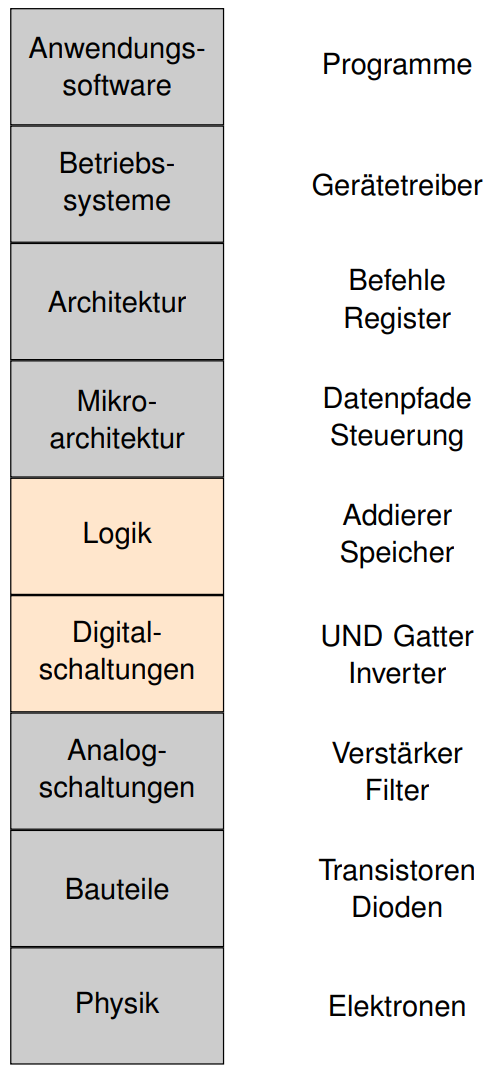
\includegraphics[height=8cm]{schichtenmodell}
		\end{figure}
	\end{minipage}
	\begin{minipage}[t]{0.7\textwidth}
		\vspace{-3.5cm}
		\begin{itemize}
		\item Untere Schicht erbringt Dienstleistungen für nächst höhere Schicht
		\item Obere Schicht nutzt nur Dienste der nächst niedrigeren Schicht
		\item Eindeutige Schnittstelle zwischen den Schichten
		\item Vorteile: 
			\begin{itemize}
			\item Austauschbarkeit einzelner Schichten
			\item Nur bearbeitende Schicht muss dem Nutzer bekannt sein
			\item Festdefinierte Funktionalität niedrigerer Schichten
			\end{itemize}
		\item Nachteile:
			\begin{itemize}
			\item ggf. geringe Leistungsfähigkeit des Systems
			\end{itemize}
		\end{itemize}
	\end{minipage}

\vspace{0.4cm}

\item \textbf{Disziplin}
	\begin{itemize}
	\item wissentliche Beschränkung der Realisierungsmöglichkeiten
	\item z.B.: Digitale Entwurfsdisziplin | Digitale Abstraktion 
		\begin{itemize}
		\item Arbeit mit diskreten statt stetigen Spannungspegeln
		\item Einfacher Entwurf $\rightarrow$ Entwurf komplexerer Schaltungen
		\end{itemize}
	\end{itemize}

\item \textbf{Wesentliche Techniken}
	\begin{itemize}
	\item Hierarch\textbf{y} | Aufteilen eines Systems in Module und Untermodule
	\item Modularit\textbf{y} | wohldefinierte Schnittstellen und Funktionen
	\item Regularit\textbf{y} | bevorzuge einfache Lösungen für einfachere Wiederverwendbarkeit
	\end{itemize} 

\item \textbf{Bits und Bytes | Digitale Abstraktion}
	\begin{itemize}
	\item Grundlagen 
		\begin{itemize}
		\item Beschränkung auf zwei unterschiedliche Werte 0 | 1
		\item Bit (binary digit) Maßeinheit für Information (kleinstmöglich)
		\item Bitfolgen $\rightarrow$ mehrere Bits hinteinander
		\item Anzahl der möglichen Zustände: $2^n$
		\item $2^5 = 32$ | $2^{10} = 1024$
		\end{itemize}		 
	
	\item Größenordnungen
	\item[] %\begin{center}
				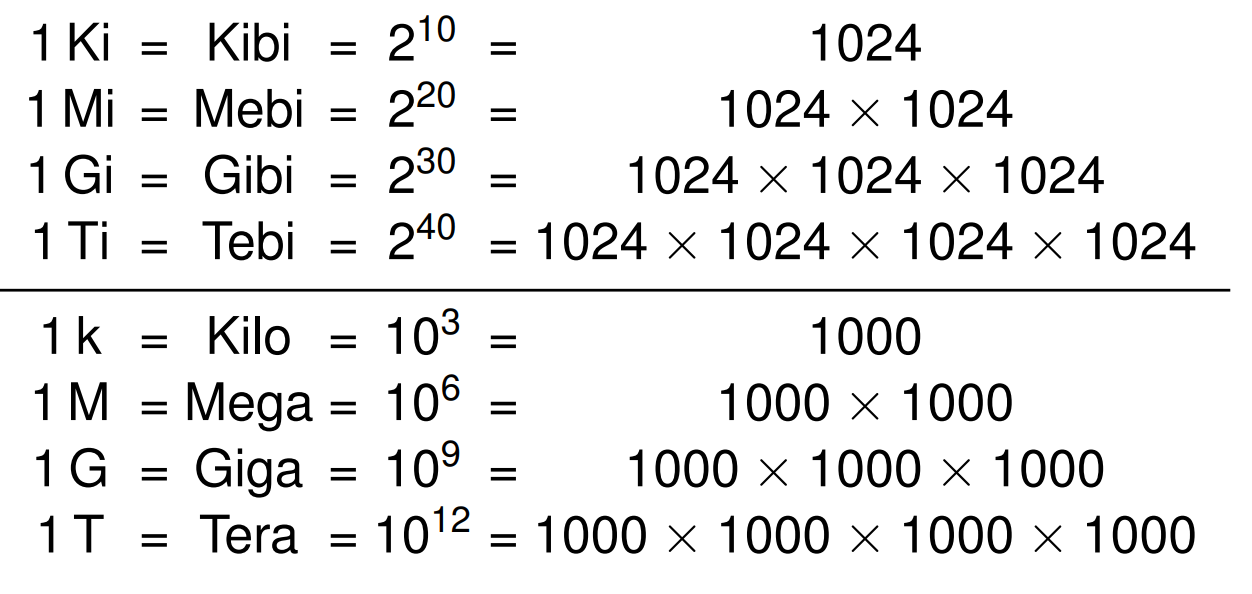
\includegraphics[height=3.5cm]{groessenordnung}
			%\end{center}	 
		
	\item Nomenklatur
		\begin{itemize}
		\item Nibble: Besteht auf 4 Bit
		\item Byte: Besteht auf 8 Bit
		\item Halbwort: Abhängig von Registerbreite (32Bit/64Bit) | Hälfte eines Worts
		\item Wort: Entspricht Registerbreite (32Bit/64Bit)
		\end{itemize}
	\end{itemize}
	
	
\end{itemize}

\subsection{Zahlensysteme}
\begin{itemize}

\item \textbf{Darstellung von natürlichen Zahlen}
	\begin{itemize}
	\item Allgemein | vorzeichenloses Stellenwertsystem
		\begin{itemize}
		\item Basis $b \in \mathbb{N} \land b \geq 2$
		\item Menge der verfügbaren Ziffern $Z_b := {0,1,..,b - 1}$
		\item $u_{b,k}$ bildet Ziffernfolge der Breite $k \in \mathbb{N}$ auf eine natürliche Zahl ab 
		\item $u_{b,k} : (a_{k-1}...a_1a_0) \in Z^k_b \rightarrow \sum^{k-1}_{i=0} a_i * b^i \in \mathbb{N}$
		\item[]
		\item polyadisches Zahlensystem $\rightarrow$ Wertigkeit von Position abhängig
		\item niedrigstwertige Stelle (\textbf{LSD}, least significant digit): $a_0$
		\item höchstwertige Stelle (\textbf{MSD}, most significant digit): $a_{k-1}$
		\item Anzahl der darstellbaren Werte: $b^k$
		\end{itemize}
	
	\item Beispiele:
		\begin{itemize}
		\item Dezimal: $302 = 3 * 100 + 0 * 10 + 2 * 1 = 302_{10}$
		\item binär: $1101_2 = 1 * 2^3 + 1 * 2^2 * 0 * 2^1 + 1 * 2^0 = 13_{10}$
		\item hexadezimal: $1F3A_16 = 1 * 16^3 + 15 * 16^2 + 3 * 16^1 + 10 * 16^0 = 7994_{10}$
		\end{itemize}
	\end{itemize}

\item \textbf{Umrechnen von Zahlensystemen}
	\begin{itemize}
	\item Binär/Hexadezimal $\rightarrow$ Dezimal
		\begin{itemize}
		\item polyadische Abbildung verwenden
		\item $u_{2,5}(1 0011_2) = 2^0 + 2^1 + 2^4 = 19_{10}$
		\item $u_{16,3}(4AF_{16}) = 15 *16^0 + 10 * 16^1 + 4 * 16^2 = 1199_{10}$
		\item (Hinweis: $16^2 = 256$ | $16^3 = 4096$)
		\end{itemize}
	
	\item Binär $\leftrightarrow$ Hexadezimal
		\begin{itemize}
		\item Nibble-weise umwandeln
		\item bei LSD beginnen 
		\item führende Nullen weglassen oder ergänzen (je nach geforderter Bitbreite)
		\item $11~1010~0110~1000_2 = 3A68_{16}$
		\item $7BF_{16} = 111~1011~1111_2$
		\end{itemize}
		
	\item Dezimal $\rightarrow$ Binär
		\begin{itemize}
		
		\item[]
			\begin{minipage}{0.3\textwidth}
				\begin{figure}[H]
				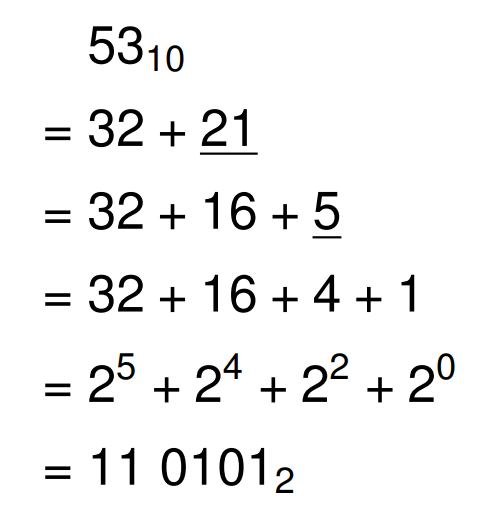
\includegraphics[height=4cm]{dtob1}
				\caption{Maximale Zweierpotenzen abziehen}
				\end{figure}
			\end{minipage}
			\begin{minipage}[t]{0.35\textwidth}
				\begin{figure}[H]
				\vspace{-3cm}
				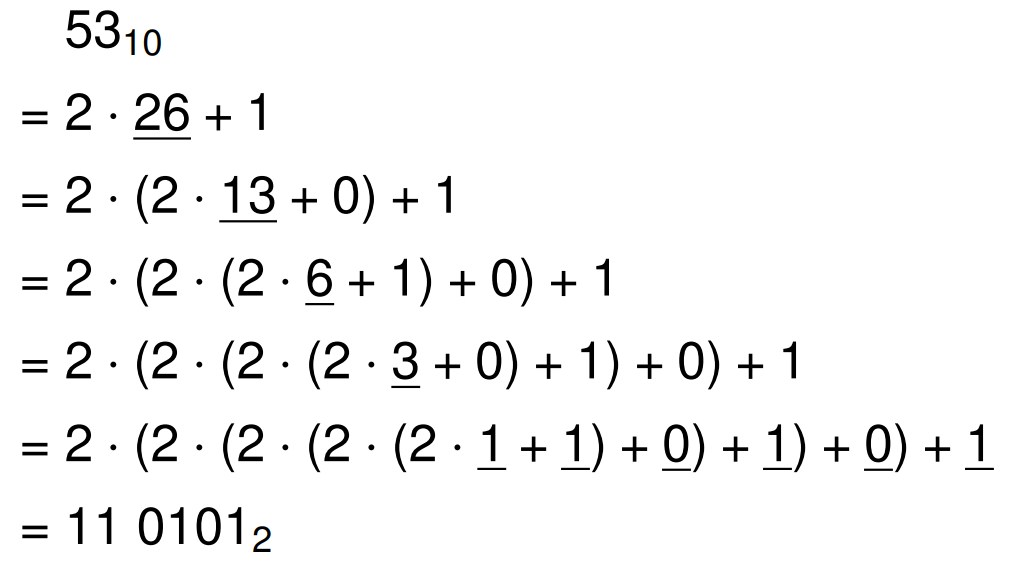
\includegraphics[height=4cm]{dtob2}
				\caption{Halbieren mit Rest}
				\end{figure}
			\end{minipage}
		
		\end{itemize}
	
	\item[] 
		\begin{figure}[H]
		\begin{center}
			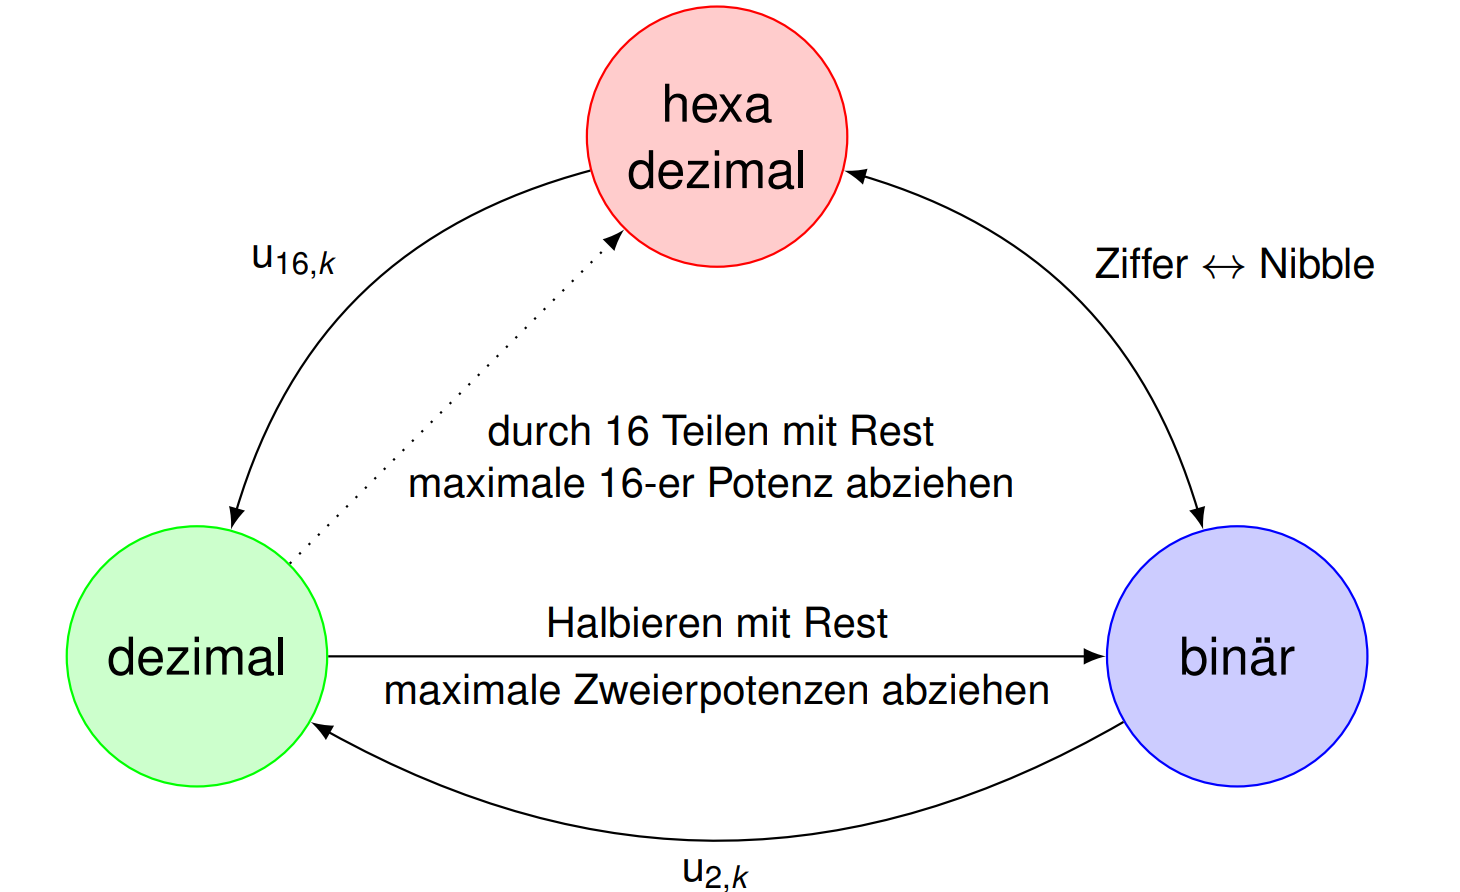
\includegraphics[height=5cm]{umwandlungoverview}
			\caption{Übersicht über Umrechnungsverfahren}
			\end{center}
		\end{figure}
	\end{itemize}

\item \textbf{Addition von vorzeichenlosen Binärzahlen}
	\begin{itemize}
	\item 
		\begin{minipage}{0.4\textwidth}
			\begin{figure}[H]
			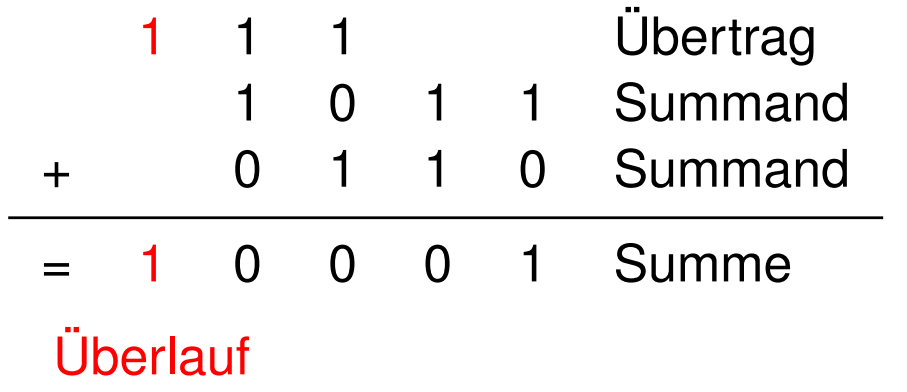
\includegraphics[height=3cm]{addoverflow}
			\end{figure}
		\end{minipage}
		\begin{minipage}[t]{0.4\textwidth}
			\vspace{-1.5cm}
			\begin{itemize}
				\item Überlauf bei festen Bitbreiten
				\item Informationsverlust!
				\item z.B.: 4-Bit Addierer $11+6=1$
			\end{itemize}
		\end{minipage}
	
	\end{itemize}

\item \textbf{Vorzeichenbehaftete Binärzahlen}
	\begin{itemize}
	\item Vorzeichen und Betrag
		\begin{itemize}
		\item Erstes Bit als Vorzeichen ($*~(-1)^1$ oder $*~(-1)^0$)
		\item z.B.: $vb_{2,4}(1110_2)=(0*2^0+1*2^1+1*2^2)*(-1)^1=-6_{10}$
		\item inkompatibel mit binärer Addition 
		\end{itemize}
		
	\item Zweierkomplement
		\begin{itemize}
		\item $s_k:(a_{k-1},...,a_1,a_0) \in \mathbb{B} \rightarrow a_{k-1} * (-2^{k-1}) + \sum^{k-2}_{i=0} a_i * 2^i \in \mathbb{Z}$
		\item Funktion $s_k$ bildet eine Bitfolge der Breite k $\in \mathbb{N}$ auf eine ganze Zahl ab
		\item Anzahl darstellbarer Werte: $2^k$
		\item Wertebereich: $\{-2^{k-1},...,2^{k-1}-1\}$
		\item z.B.: $s_4(1010_2) = 0*2^0+1*2^1+0*2^2+1*(-2^3)=-6_{10}$
		\item kompatibel mit binärer Addition
		\end{itemize}			
	
	\item Dezimal $\rightarrow$ Zweierkomplement
		\begin{itemize}
		\item in beiden Fallen achten auf korrekte/geforderte Bitbreite 
		\item ggf. führende Nullen vor Betragsdarstellung
		\item[]
			\begin{minipage}{0.4\textwidth}
				\begin{figure}[H]
				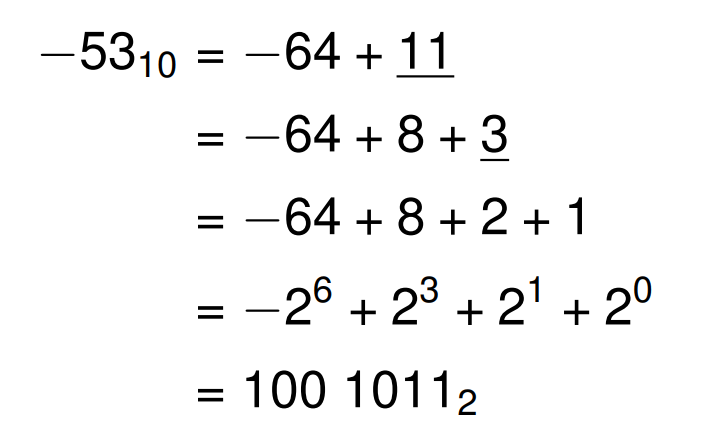
\includegraphics[height=4cm]{dtoz1}
				\caption{Maximale Zweierpotenzen abziehen}
				\end{figure}
			\end{minipage}
			\begin{minipage}[t]{0.45\textwidth}
				\begin{figure}[H]
				\vspace{-3cm}
				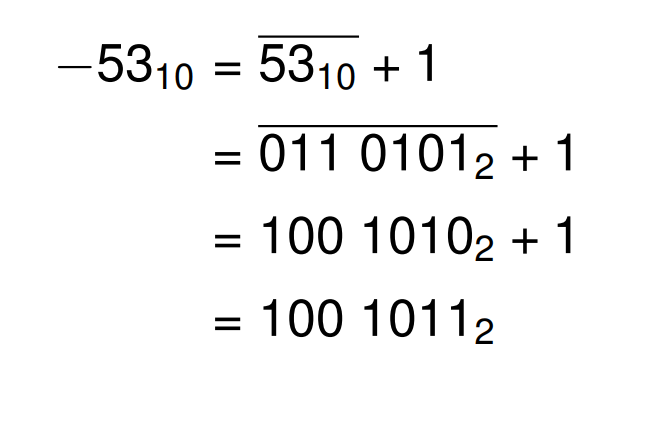
\includegraphics[height=4cm]{dtoz2}
				\caption{Negieren und Inkrement(+1)}
				\end{figure}
			\end{minipage}
		
		\end{itemize}
	\end{itemize}
	
	\pagebreak	
	
\item \textbf{Bitbreitenerweiterung}
	\begin{itemize}
	\item Notwendig für Addition verschiedener Bitbreiten
	\item zero extension: Auffüllen mit führenden Nullen für vorzeichenlose Darstellung
	\item sign extension: Auffüllen mit Wert des Vorzeichen-Bits für Zweierkomplement-Darstellung
	\item z.B.: Falls in Aufgaben eine Bitbreite von 8Bit gefordert wird
	\end{itemize}

\item \textbf{Vergleich der binären Zahlendarstellungen}
\item[] \begin{figure}[H]
			\begin{center}
			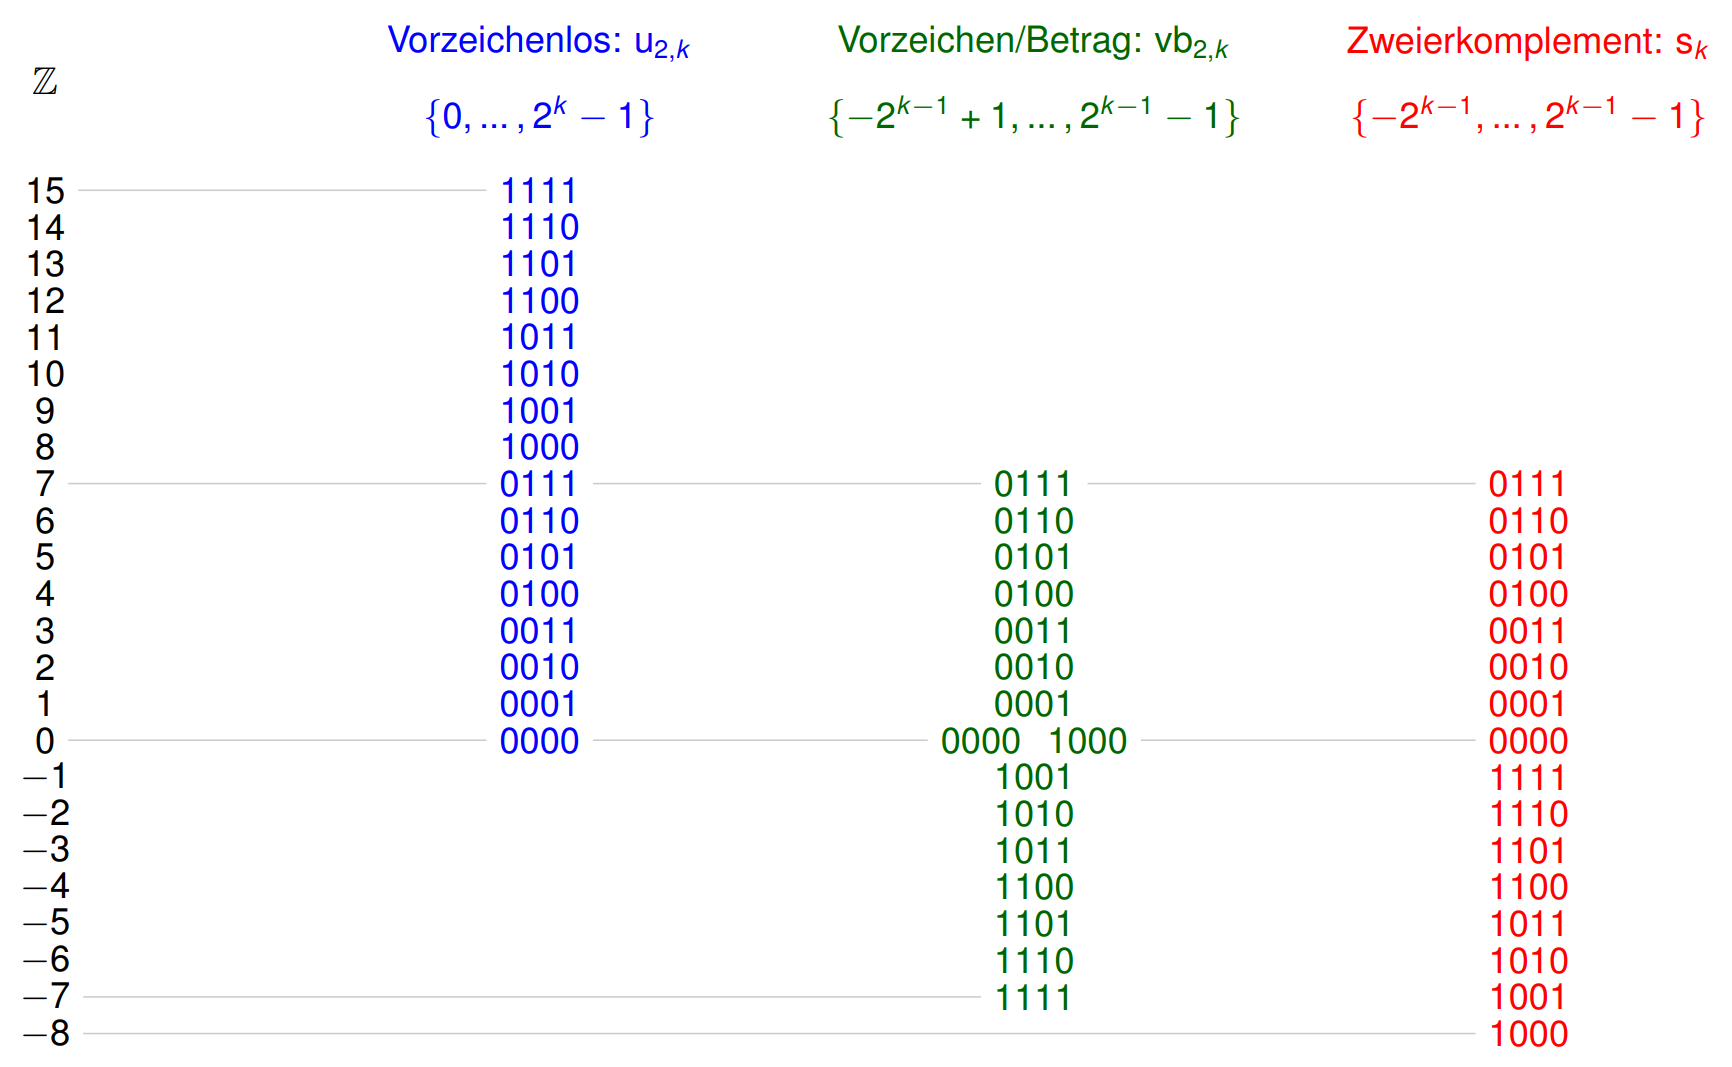
\includegraphics[height=5cm]{compzahlen}
			\end{center}
		\end{figure}

\end{itemize}

\subsection{Logikgatter}
\begin{itemize}

\item \textbf{Logische Operationen}
	\begin{itemize}
	\item verknüpfen binäre Werte $\mathbb{B}^n \rightarrow \mathbb{B}^k$
	\item Charakterisierung durch Wahrheitstabellen
	\item z.B.: $n = 1: NOT$ | $n = 2: AND, OR,XOR$ | $n = 3: MUX$
	\end{itemize}

\item \textbf{Gatterarten auf Merkblatt}

\item \textbf{Fehlerkorrektur mit Paritätsfunktion}
	\begin{itemize}
	\item $Y = 1$, falls Anzahl an eingehenden Einsen ungerade
	\item Verwendung in Fehlerkorrektur bei Übertragung
	\item 1. Anhängen eines Paritätsbits 
	\item 2. Gesamtparität nach Übertragung berechnen
	\item Verwendung von mehreren Paritätsbits für Nachricht für Fehlerkorrektur
	\item[] 	
		\begin{figure}[H]
		\begin{center}
		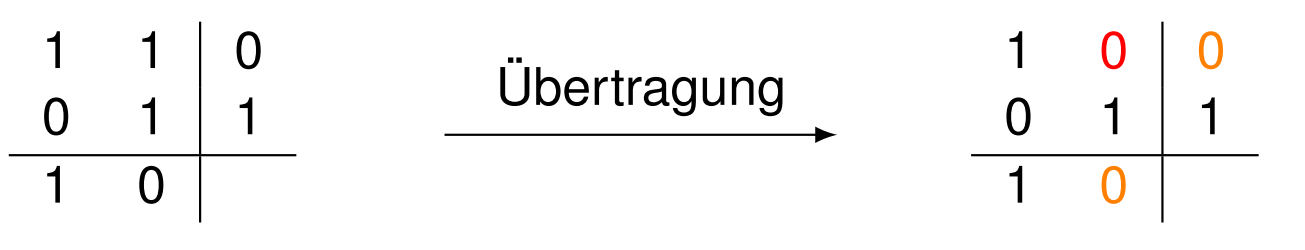
\includegraphics[height=3cm]{fehlerpari}
		\end{center}
		\end{figure}
	\end{itemize}

\end{itemize}

\pagebreak

\subsection{MOSFET Transistoren und CMOS Gatter}
\begin{itemize}

\item \textbf{Spannungen als Logikpegel}
	\begin{itemize}
	\item Definition von Logikpegeln für 0 und 1
	\item $0V \rightarrow 0$ (GND, Voltage Source Source ($V_{SS}$))
	\item $5V \rightarrow 1$ (Versorgungsspannung, Voltage Drain Drain ($V_{DD}$))
	\item[]
	\item Definition von Spannungsbereichen aufgrund von Rauschen (z.B. Widerstände)
		\begin{itemize}
		\item $V_{IL}$: größte Spannung, die Empfänger als 0 interpretiert (Voltage Input Low)
		\item $V_{IH}$: kleinste Spannung, die Empfänger als 1 interpretiert (Voltage Input High)
		\item $V_{OL}$: größte Spannung, die Treiber als 0 ausgibt (Voltage Output Low)
		\item $V_{OH}$: kleinste Spannung, die Treiber als 1 ausgibt (Voltage Output High)
		\item $NM_H= V_{OH} - V_{IH}$: oberer Störabstand (Noise Margin High)
		\item $NM_L = V_{IL} - V_{OL}$: unterer Störabstand (Noise Margin Low)
		\item[] \begin{figure}[H]
				\begin{center}
				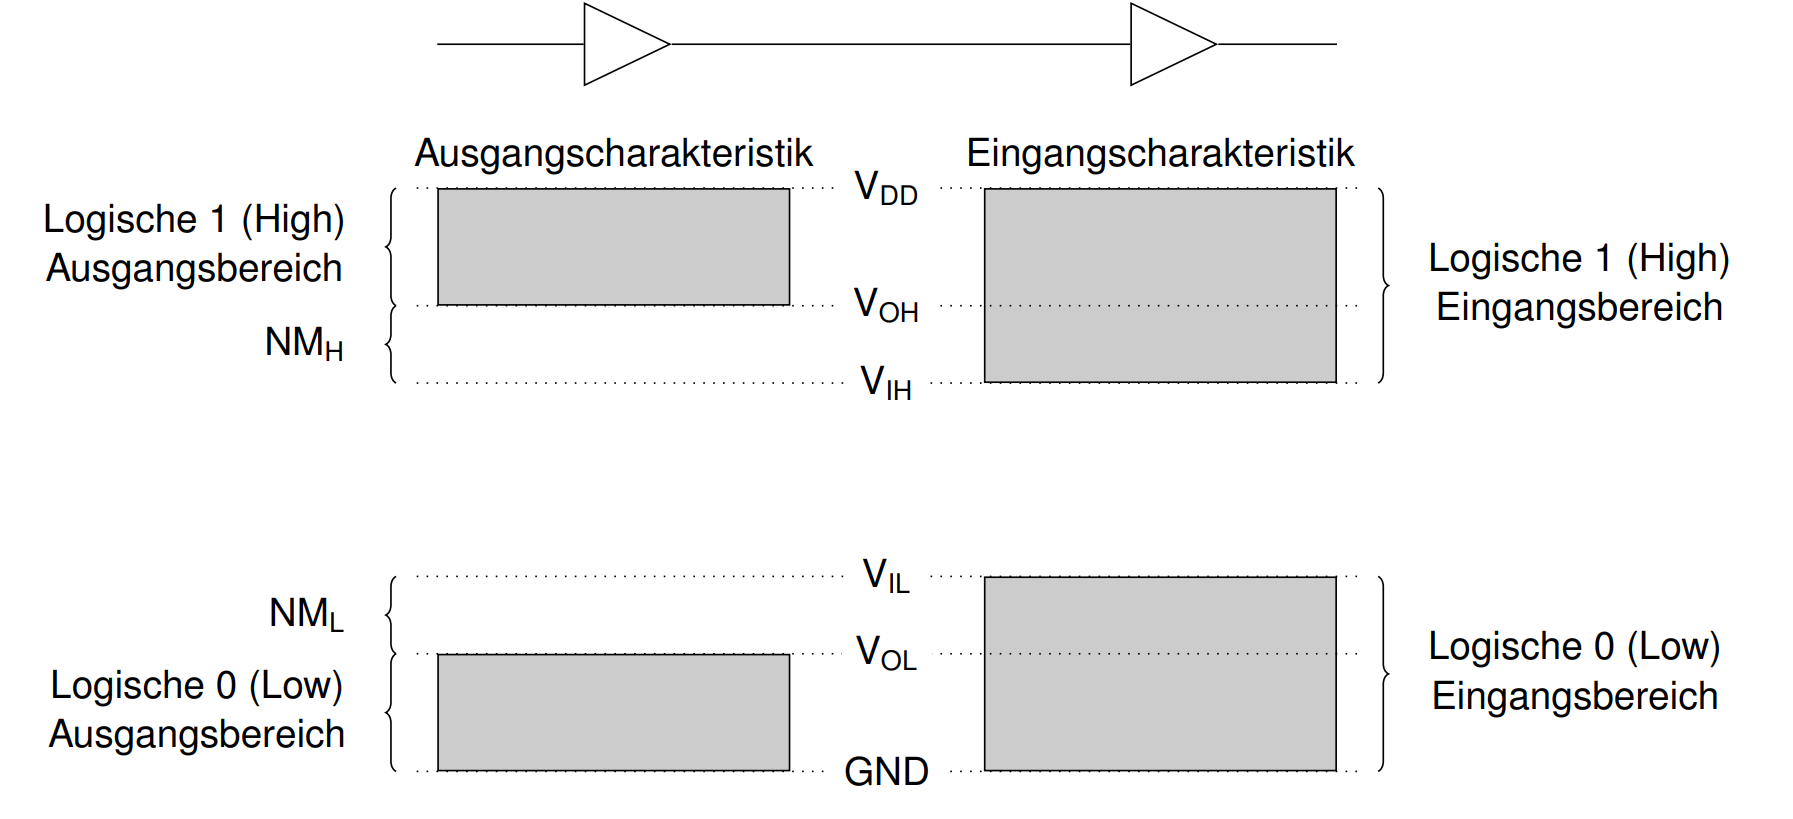
\includegraphics[height=4cm]{spannungsbereiche}
				\end{center}
				\end{figure}
		\end{itemize}
	\end{itemize}

\item \textbf{Feldeffekt-Transistoren}
	\begin{itemize}
	\item Logikgatter werden aus Transistoren aufgebaut (heutzutage hauptsächlich FET)
	\item Transistor: 
		\begin{itemize}
		\item Spannungsgesteuerte Schalter
		\item Zwei Anschlüsse werden je nach Spannung am 3. Eingang (Gate) getrennt oder verbunden
		\end{itemize}			
	\item Der Feldeffekt
		\begin{itemize}
		\item Prinzip des spannungsgesteuerten Widerstands
		\item[] \begin{figure}[H]
				\begin{center}
				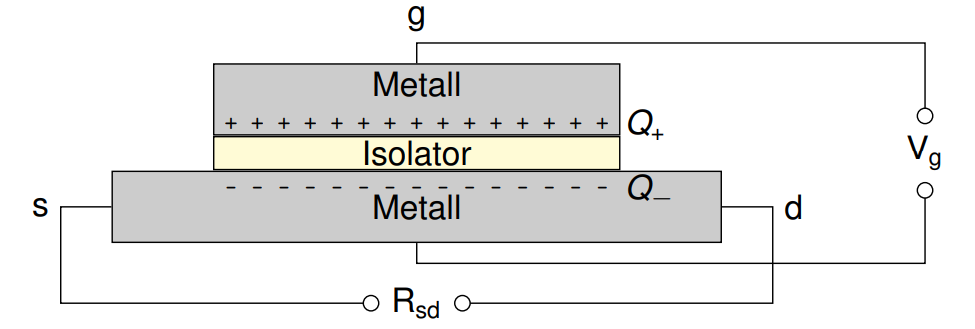
\includegraphics[height=2.5cm]{feldeffekt}
				\end{center}
				\end{figure}
		\item Metallische Streifen bilden Plattenkondensator
		\item Steuerspannung $V_g$ beeinflusst Menge der freien Ladungsträger
		\item Steuerung des Widerstands $R_{sd}$ mithilfe der Steuerspannung $V_g$ 
		\item Nutzung von Halbleitern, da der Feldeffekt dort technisch nutzbar
		\item meist dotierte Silizium-basierte Halbleiter
		\end{itemize}
		
	\item MOSFETs
		\begin{itemize}
		\item Metalloxid-Halbleiter (MOS) Transistoren
		\item Undotiertes Silizium als Gate
		\item Oxid (Siliziumdioxid) als Isolator
		\item Dotiertes Silizium als Substrat und Anschlüsse
		\item[] \begin{figure}[H]
				\begin{center}
				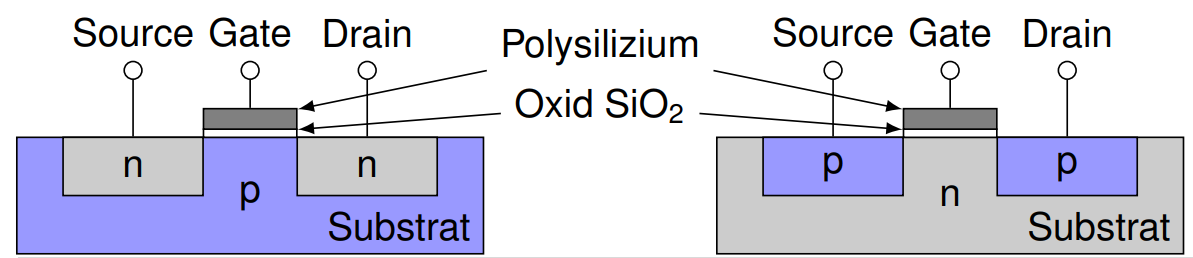
\includegraphics[height=2.5cm]{npmos}
				\caption{Links: nMOS | Rechts: pMOS}
				\end{center}
				\end{figure}
		\item nMOS: $Gate = 0 \rightarrow AUS ~~~ Gate = 1 \rightarrow AN$
		\item pMOS: $Gate = 0 \rightarrow AN ~~~ Gate = 1 \rightarrow AUS$
		\item[]
			\begin{minipage}{0.3\textwidth}
				\begin{figure}[H]
				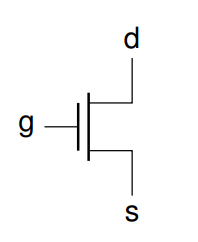
\includegraphics[height=4cm]{nmos}
				\caption{nMOS}
				\end{figure}
			\end{minipage}
			\begin{minipage}[t]{0.4\textwidth}
				\begin{figure}[H]
				\vspace{-2.75cm}
				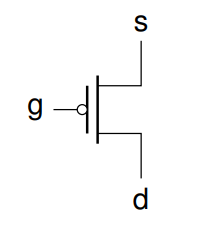
\includegraphics[height=4cm]{pmos}
				\caption{pMOS (Kreis wie im p)}
				\end{figure}
			\end{minipage}
		\end{itemize}
	\end{itemize}


\item \textbf{CMOS-Gatter}
	\begin{itemize}
		\item[]		
			\begin{minipage}{0.3\textwidth}
				\begin{figure}[H]
				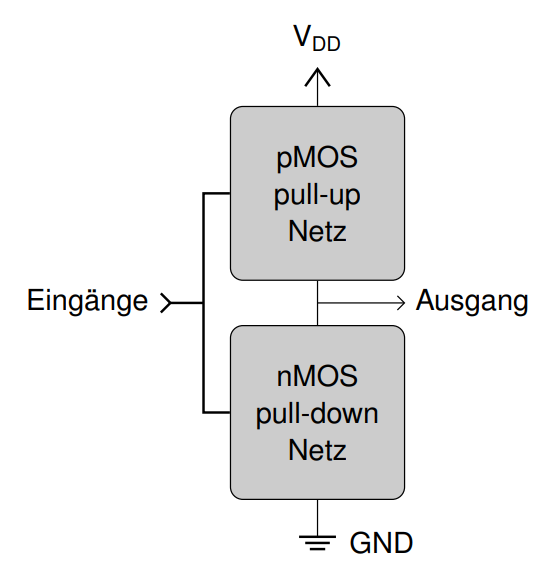
\includegraphics[height=5cm]{cmos}
				\end{figure}
			\end{minipage}
			\begin{minipage}[t]{0.7\textwidth}
				\vspace{-1.25cm}
				\begin{itemize}
				\item Kombinieren von komplementären Transistoren
				\item nMOS leiten 0'en gut weiter $\rightarrow$ Source an GND anschließen
				\item pMOS leiten 1'en gut weiter $\rightarrow$ Source an $V_{DD}$ anschließen
				\item[$\Rightarrow$] Complementary Metal-Oxide-Semiconductor sn(CMOS) Logik
				\end{itemize}
			\end{minipage}	
		
		\item Struktur: 
			\begin{itemize}
			\item pMOS Parallelschaltung $\Leftrightarrow$ nMos Serienschaltung
			\item nMOS Parallelschaltung $\Leftrightarrow$ pMos Serienschaltung
			\end{itemize}
		
		\item Pseudo-nMOS Gatter
			\begin{itemize}
			\item[]		
				\begin{minipage}{0.25\textwidth}
					\begin{figure}[H]
					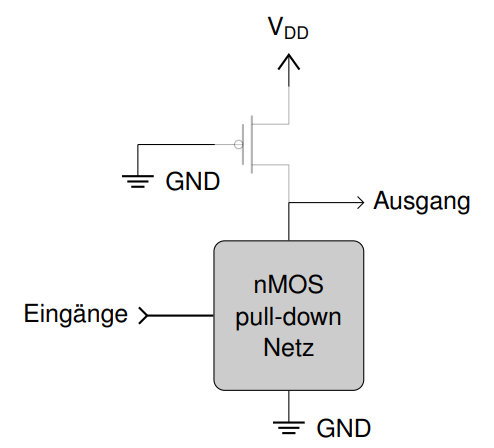
\includegraphics[height=4cm]{pseudonmos}
					\end{figure}
				\end{minipage}
				\begin{minipage}[t]{0.6\textwidth}
					\vspace{-1.25cm}
					\begin{itemize}
					\item Ersetzt das pMOS-Pull-Up-Netz
					\item[$\rightarrow$] durch schwachen, immer eingeschalteten pMOS
					\item Pull-Up kann durch Pull-Down überstimmt werden
					\end{itemize}
				\end{minipage}
			\end{itemize}
		\item Transmissionsgatter
			\begin{itemize}
			\item[]		
				\begin{minipage}{0.25\textwidth}
					\begin{figure}[H]
					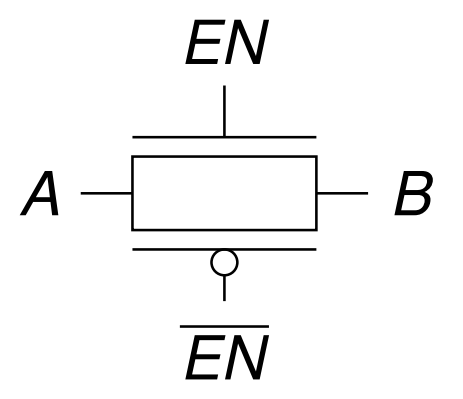
\includegraphics[height=4cm]{tgates}
					\end{figure}
				\end{minipage}
				\begin{minipage}[t]{0.6\textwidth}
					\vspace{-1.25cm}
					\begin{itemize}
					\item besseres Schalter $\Rightarrow$ leitet 0 und 1 gut weiter
					\item $EN = 1 ~ und ~ \overline{EN}=0 \Rightarrow$ EIN (A mit B verbunden)
					\item $EN = 0 ~ und ~ \overline{EN}=1 \Rightarrow$ AUS (A nicht mit B verbunden)
					\end{itemize}
				\end{minipage}
			\end{itemize}
	\end{itemize}


\end{itemize}
\subsection{Leistungsaufnahme}
\begin{itemize}
\item \textbf{Leistung} = Energieumsatz/-verbrauch pro Zeiteinheit

\item \textbf{Statische Leistungsaufnahme:} 
	\begin{itemize}
	\item Leistungsbedarf wenn kein Gatter schaltet
	\item verursacht durch Leckstrom $I_{DD}$ (nicht vollständiges Abschalten, Pseudo-nMOS,...)
	\item $P_{static} = I_{DD} * V_{DD}$
	\end{itemize}

\item \textbf{Dynamische Leistungsaufnahme:} 
	\begin{itemize}
	\item Aufladen der Gate-Kapazität $C$ von $0 As$ auf $Q = C * V_{DD}$
	\item Schaltung wird mit Frequenz $f$ betrieben $\Rightarrow$ Transistoren schalten $f$-mal pro Sekunde
	\item Nur die Hälfte davon sind Aufladungen
	\item $P_{dynamic} = I * V = \frac{1}{2} C*V_{DD}^2*f$
	\item Beispiel Leistungsaufnahme:
	\item[]	\vspace{-0.35cm}
			\begin{figure}[H]
				\begin{center}
				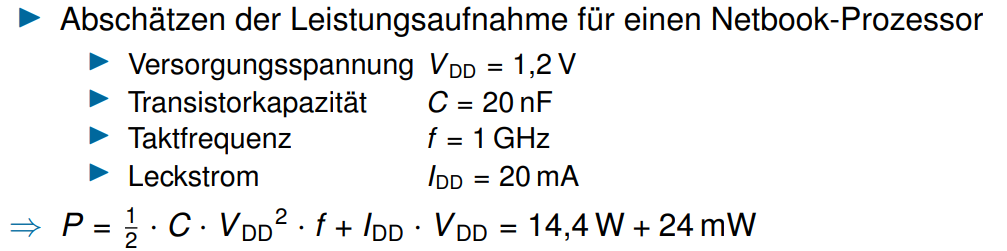
\includegraphics[height=3cm]{bspleistung}
				\end{center}
			\end{figure}
	\end{itemize}
	
\item \textbf{Moore'sches Gesetz} (Alle 18 Monate verdoppelt sich die Anzahl der Transistoren auf einem Chip)
	
	
\end{itemize}
%--------------------------------------------------------------------------------

\section{Kombinatorische Schaltungen}
\subsection{Boole'sche Gleichungen und Algebra}
\begin{itemize}
\item \textbf{Kombinatorische Logik}
	\begin{itemize}
	\item Eingänge führen durch bestimmtes Verhalten zu Ausgängen (Funktionales und Zeitverhalten)
	\item kombinatorische Logik $\Rightarrow$ hängt nur von Eingangswerten ab
	\item sequentielle Logik $\Rightarrow$ hängt von Eingangswerten und internem Zustand ab
	\item Eigenschaften:
		\begin{itemize}
		\item Jedes Schaltungselement ist selbst kombinatorisch
		\item Jeder Pfad besucht jeden Knoten maximal einmal (zyklenfrei)
		\end{itemize}
	\end{itemize}
	
\item \textbf{Bool'sche Gleichungen}
	\begin{itemize}
	\item Grundlagen:
		\begin{itemize}
		\item beschreiben Ausgänge als Funktion der Eingänge $\Rightarrow$ Spezifikation des funktionalen Verhaltens
		\item Operatoren: (sortiert nach Operatorpräzedenz)
			\begin{itemize}
			\item NOT: $\overline{A}$
			\item AND: $A~B=A*B$
			\item XOR: $A \oplus B$
			\item OR: $A+B$
			\end{itemize}
		\item Komplement: Intervierte boole'sche Variable $(\overline{A})$
		\item Literal: Variable oder ihr Komplement$(A, \overline{A})$
		\item Impliktant: Produkt von Literalen $(ABC)$
		\item Minterm: Produkt (UND, Konjunktion) über alle Eingangsvariablen $(ABC)$
		\item Maxterm: Summe (ODER, Disjunktion) über alle Eingangsvariablen $(A+B+C)$
		\end{itemize}
		
	 \item Minterm:
	 	\begin{itemize}
	 	\item Produkt, das jede Eingangsvariable genau einmal enthält
	 	\item einspricht einer Zeile in Wahrheitstabelle
	 	\item Jeder Minterm wird für genau eine Eingangskombination \textbf{wahr}
	 	\item Disjunktive Normalform(DNF) = Sum-Of-Products(SOP)
	 		\begin{itemize}
	 		\item Summe aller Minterme, für welche die \textbf{Funktion wahr} ist $\Rightarrow$ nur eine DNF
	 		\item z.B.: $Y = m_1+m_2= \overline{A}~B + A ~ \overline{B}$
	 		\end{itemize}
		\end{itemize}	 		
	
	\item Maxterm:
		\begin{itemize}
	 	\item Produkt, das jede Eingangsvariable genau einmal enthält
	 	\item einspricht einer Zeile in Wahrheitstabelle
	 	\item Jeder Maxterm wird für genau eine Eingangskombination \textbf{falsch}
	 	\item Konjunktive Normalform(KNF) = Product-of-sums (POS)
	 		\begin{itemize}
	 		\item Produkt aller Maxterme, für welche die \textbf{Funktion falsch} ist $\Rightarrow$ nur eine KNF
	 		\item z.B.: $Y=M_0~M_3=(A+B)(\overline{A} + \overline{B})$
	 		\end{itemize}
		\end{itemize}
	

	\end{itemize}
	
\item \textbf{Boole'sche Algebra}
	\begin{itemize}
	\item Axiome: grundlegende Annahmen der Algebra (nicht beweisbar)
	\item Theoreme: komplexere Regeln, die sich aus Axiomen ergeben (beweisbar)
	\item Optimierungen durch Begrenzung auf $\mathbb{B}$
	\item Axiome und Theoreme zu finden auf Hilfsblatt
	\end{itemize}
	
\item \textbf{Logikminimierung}
	\begin{itemize}
	\item TO-DO (Übungen)
	
	\item Bubble-Pushing
		\begin{itemize}
		
		\item Verschieben von Invertierungsblasen zur Vereinfachung von Schaltern
		\item Über Gatter hinweg $\Rightarrow$ De Morgan | And $\Leftrightarrow$ OR | Verschieben der Blasen
		\item Zwischen Gattern $\Rightarrow$ Über Leitungen | Involution (doppelte Blasen) 
		\item Entfernen verbleibender Buffer
		
		\end{itemize}
	\end{itemize}
	
\end{itemize}

\subsection{Kombinatorische Grundelemente}
\begin{itemize}

\item \textbf{Zweistufige Logik}
	\begin{itemize}
	\item direkte Umsetzung der disjunktiven Normalform (DNF)
	\item aufwändige Darstellung und Realisierung
	\item Eingangsliterale: Ein Inverter pro Variable
	\item Minterme: Je ein AND Gatter an passende Literale anschließen
	\item Summe: ALle Minterme an ein OR Gatter anschließen
	\item[$\Rightarrow$] jede boole'sche Funktion mit Basisgattern realisierbar
	\item z.B.:
	\item[] \begin{figure}[H]
				\begin{center}
				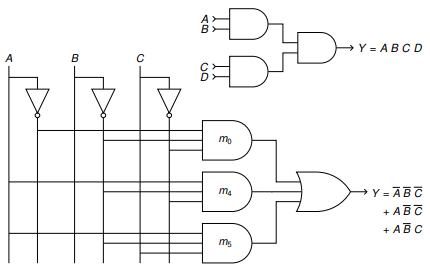
\includegraphics[height=4cm]{zweistufigelogik}
				\end{center}
			\end{figure}
	\end{itemize}

\item \textbf{Konventionen für Schaltpläne}
	\begin{itemize}
	\item Eingänge links/oben | Ausgänge rechts/unten
	\item gerade und rechtwinklige Verbindungen
	\item[] \begin{figure}[H]
				\begin{center}
				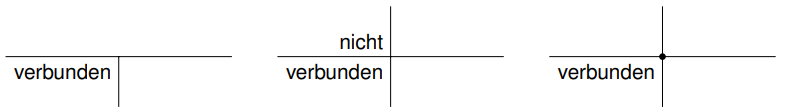
\includegraphics[height=2cm]{konventionen}
				\end{center}
			\end{figure}
	\end{itemize}

\item \textbf{Multiplexer $MUXn: \mathbb{B}^{n+[log_2n]} \rightarrow \mathbb{B}$}
	\begin{itemize}
	\item Selektiert einen der Datenausgänge $A_0,...,A_n-1$ als Ausgang $Y$
	\item $k = [log_2n]$ Steuersignale $S_0,...,S_{k-1}$
	\item $Y= A_{u_{2,k}}(S_{k-1}...S_0)$
	\item[] \begin{figure}[H]
				\begin{center}
				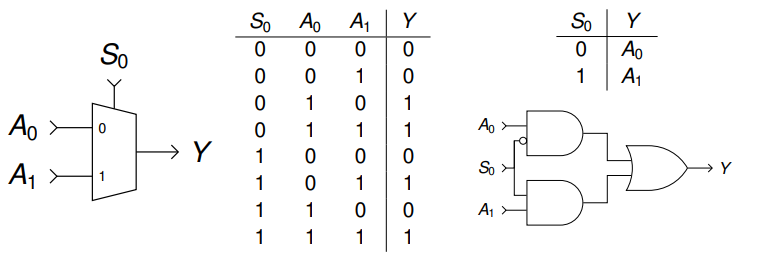
\includegraphics[height=4cm]{multiplexer}
				\end{center}
			\end{figure}
	\end{itemize}
	
\item \textbf{Dekodierer $DECODEn: \mathbb{B}^n \rightarrow \mathbb{B}^{2^n}$}
	\begin{itemize}
	\item $n$ Eingänge $A_0,...,A_{n-1}$
	\item $2^n$ Ausgänge $Y_0,...,Y_{2^n-1}$
	\item $Y_i = u_{2,n}(A_{n-1}...A_0) == i~?~ 1:0$ (''One-Hot'' Kodierung)
	\item[] \begin{figure}[H]
				\begin{center}
				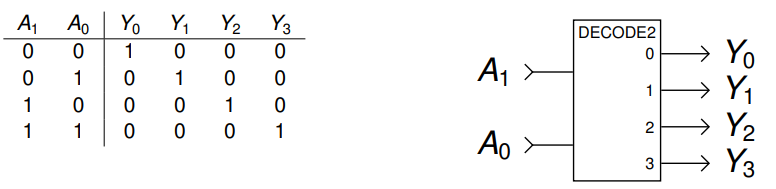
\includegraphics[height=2cm]{dekodierer}
				\end{center}
			\end{figure}
	\item Logikrealisierung: Summe über Minterme, auf denen Zielfunktion wahr ist
	\item[$\Rightarrow$] Decoder ersetzt erste Stufe der zweistufigen Logikrealisierung
	\item[] \begin{figure}[H]
				\begin{center}
				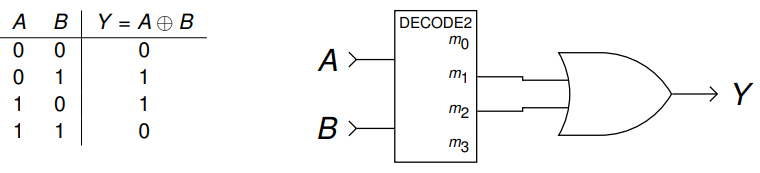
\includegraphics[height=2cm]{dekodierer2}
				\end{center}
			\end{figure}
	\end{itemize}

\end{itemize}

\subsection{Karnaugh-Diagramme (KV)}
\begin{itemize}

\item \textbf{Allgemein}
	\begin{itemize}
	\item Minimierung boole'scher Ausdrücke durch Zusammenfassen von Mintermen
	\item $Y = AB +A\overline{B}= A$
	\item[$\Rightarrow$] Graphische Darstellung der Zusammenhänge durch Karnaugh-Diagramme
	\item via GrayCode (immer nur ein geändertes Bit nebeneinander)
	\item Zusammenhängende Minterme dadurch besser erkennbar
	\item Don't Cares sowohl in DNF als auch KNF
	\end{itemize}

\item \textbf{Beispiel für vier Eingänge}
	\item[] \begin{figure}[H]
				\begin{center}
				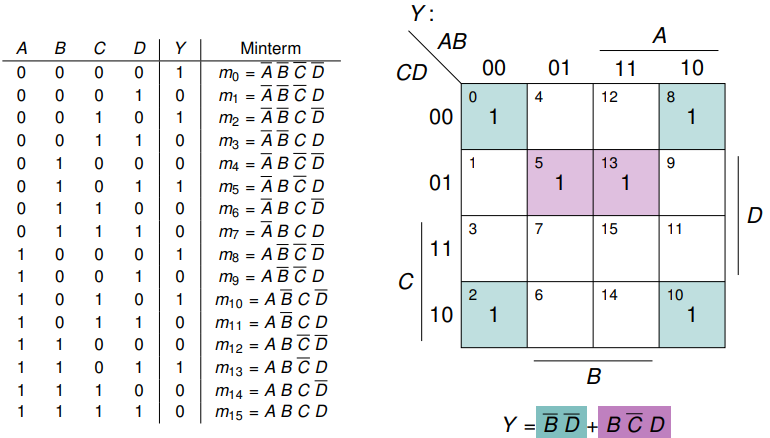
\includegraphics[height=6cm]{karnaugh4}
				\end{center}
			\end{figure}
			
\item \textbf{Minimierungsregeln}
	\begin{itemize}
	\item Eintragen von Mintermen (Einsen aus Tabelle und ''Don't cares'' (*))
	\item Markieren von Implikanten
		\begin{itemize}
		\item Bereiche dürfen nur 1 und * enthalten
		\item nur Rechtecke mit $2^k$ Einträgen
		\item Dürfen um Ränder herum reichen
		\item Müssen so groß wie möglich sein (Primimplikanten)
		\end{itemize}
	\item Ziel: Überdeckung aller Einsen mit möglichst wenigen Primimplikanten
	\end{itemize}
	\item[] \begin{figure}[H]
				\begin{center}
				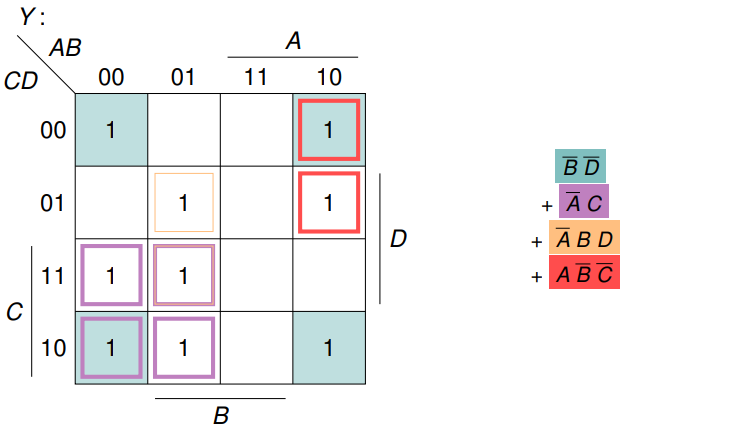
\includegraphics[height=6cm]{karnaugh42}
				\end{center}
			\end{figure}
			


\end{itemize}

\pagebreak

\subsection{Minimierung von Ausdrücken}
\begin{itemize}

\item \textbf{Ziel:} Minimiere Anzahl der zur Darstellung einer Funktion notwendigen Implikanten

\item \textbf{Espresso-Heuristik}
	\begin{itemize}
	
	\item Keywords:
		\begin{itemize}
		\item .i: Anzahl $n_i$ der Eingänge (erforderlich)
		\item .o: Anzahl $n_o$ der Ausgänge (erforderlich)
		\item .p: Anzahl der Tabellenzeilen
		\end{itemize}
	
	\end{itemize}

\end{itemize}

\subsection{Vierwertige Logik (0,1,X,Z)}
\begin{itemize}

\item \textbf{Allgemein}
	\begin{itemize}
	\item Unterscheidung von zwei weiteren Logikwerten neben 0 und 1
	\item X mehrfach getrieben: fehlerhaft
	\item Z ungetrieben/hochohmig: gezielt (high impedance)
	\item Nicht mit ''Don't care'' verwechseln
	\end{itemize}

\item \textbf{X (mehrfach getrieben): Konkurrierende Ausgänge}
	\begin{itemize}
	\item mehrere Treiber für den selben Schaltungsknoten
	\item Konflikt, sobald Treiber in entgegengesetzte Richtung ziehen
	\item Meist Entwurfsfehler (Doppelzuweisung in Verilog)
	\item[] \begin{figure}[H]
				\begin{center}
				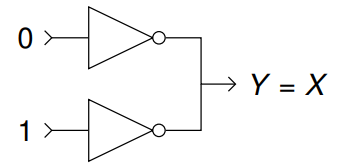
\includegraphics[height=2cm]{mehrx}
				\end{center}
			\end{figure}
	\end{itemize}
	
\item \textbf{Z (ungetrieben/hochohmig): Tristate-Buffer}
	\begin{itemize}
	\item Zusätzliches Enable-Signal EN für Buffer
	\item EN = 1: Funktion wie normaler Buffer
	\item EN = 0: Ausgang hochohmig $\rightarrow$ Z
	\item[] \begin{figure}[H]
				\begin{center}
				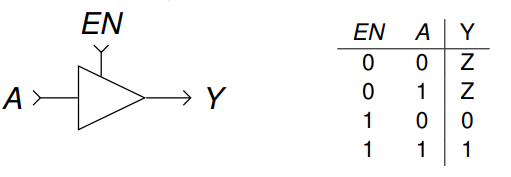
\includegraphics[height=2cm]{mehrz}
				\end{center}
			\end{figure}
	\item Verwendungin Bussen zur Zuschaltung von nur einem Treiber zur selben Zeit
	\end{itemize}
	
\item \textbf{Mehrwertige Logik in Schaltnetzen}
\item[] \begin{figure}[H]
				\begin{center}
				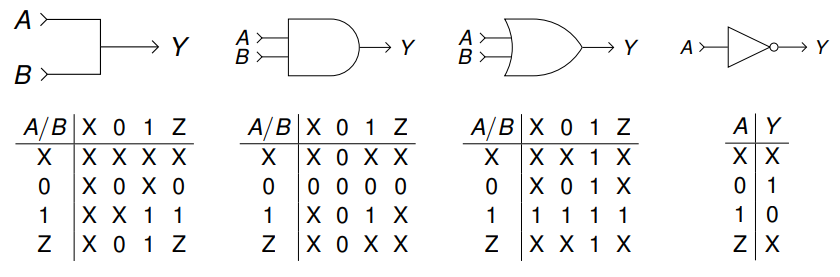
\includegraphics[height=3.5cm]{mehrTabelle}
				\end{center}
			\end{figure}


\end{itemize}

\subsection{Zeitverhalten}
\begin{itemize}

\item \textbf{Allgemein}
	\begin{itemize}
	\item reale Schaltungselemente benötigen Zeit um Änderung vom Eingang auf Ausgang zu übertragen
	\item Eingang kann Ausgang über verschiedene Pfade beeinflussen
	\item Führt zu Verzögerungen
	\end{itemize}
	
\item \textbf{Verzögerungen}
	\begin{itemize}
	\item Ausbreitungsverzögerung $t_{pd}$: Maximale Zeit vom Eingang zum Ausgang
	\item Kontaminationsverzlgerung $t_{cd}$: Minimale Zeit vom Eingang zum Ausgang
	\item[] \begin{figure}[H]
				\begin{center}
				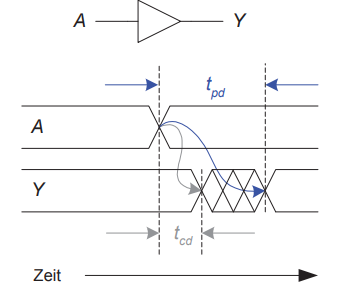
\includegraphics[height=4cm]{delays1}
				\end{center}
			\end{figure}
	\item Kritischer Pfad: Längster Pfad durch Schaltung
	\item Kurzer Pfad: Kürzester Pfad durch Schaltung	
	\end{itemize}

\item \textbf{Glitches}
	\begin{itemize}
	\item eine Änderung des Eingangs verursacht mehrere Änderungen des Ausgangs
	\item Können durch geeignete Entwurfsdisziplin entschärft werden
	\item Erkennen in Karnaugh-Diagrammen:
		\begin{itemize}
		\item Nebeneinanderliegende Einsen, die nicht zwingend verbunden werden müssen
		\item[$\rightarrow$] Überdeckung der Stelle mit zusätzlichem Implikanten
		\end{itemize}
	\end{itemize}

\end{itemize}

%--------------------------------------------------------------------------------

\section{Sequentielle Schaltungen}
\subsection{Allgemein}

\begin{itemize}
\item Ausgänge hängen von aktuellen und vorherigen Eingabewerten ab
\item sequentielle Schaltungen speichern internen Zustand
	\begin{itemize}
	\item[$\rightarrow$] realisiert durch Rückkopplungen von Ausgängen
	\end{itemize}

\item Zeitverhalten besser kontrollierbar als bei Kombinatorischen
\end{itemize}

\subsection{Latches}
\begin{itemize}

\item \textbf{Bistabile Grundschaltung}
	\begin{itemize}
	
	
	\item[]		
				\begin{minipage}{0.25\textwidth}
					\begin{figure}[H]
					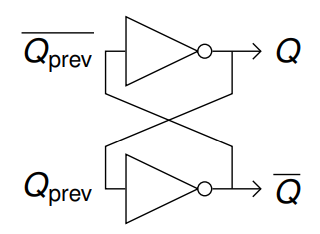
\includegraphics[height=3cm]{bistabil}
					\end{figure}
				\end{minipage}
				\begin{minipage}[t]{0.6\textwidth}
					\vspace{-1.5cm}
					\begin{itemize}
					\item Grundlage des Zustandsspeichers
					\item zwei Inverter mit Rückkopplung
					\item Speichert 1 Bit durch zwei stabile Zustände
					\item $Q=0 \Rightarrow \overline{Q} =1 \Rightarrow Q=0$
					\item $Q=1 \Rightarrow \overline{Q} =0 \Rightarrow Q=1$
					\item Keine Einflüsse auf gespeicherten Zustand
					\end{itemize}
				\end{minipage}
	
	\end{itemize}
	
\item \textbf{SR-Latch}
	\begin{itemize}
	\item[]		
				\begin{minipage}{0.25\textwidth}
					\begin{figure}[H]
					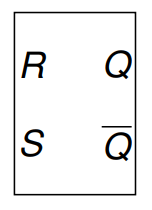
\includegraphics[height=3cm]{srlatch1}
					\end{figure}
				\end{minipage}
				\begin{minipage}[t]{0.6\textwidth}
					\vspace{-1.25cm}
					\begin{itemize}
					\item bistabile Grundschaltung mit NOR statt NOT
					\item NOR: Ausgang 0 wenn einer der Inputs 1 ist
					\item $\overline{S}~\overline{R} \rightarrow$ Zustand halten (latch = verriegeln)
					\item $\overline{S}~R \rightarrow$ Zustand 0 rücksetzen (reset $R$)
					\item $S~\overline{R} \rightarrow$ Zustand auf 1 setzen (set $S$)
					\item $S~R \rightarrow$ ungültiger Zustand ($Q=\overline{Q}=0)$
					\end{itemize}
				\end{minipage}
				
	\item[] \begin{figure}[H]
				\begin{center}
				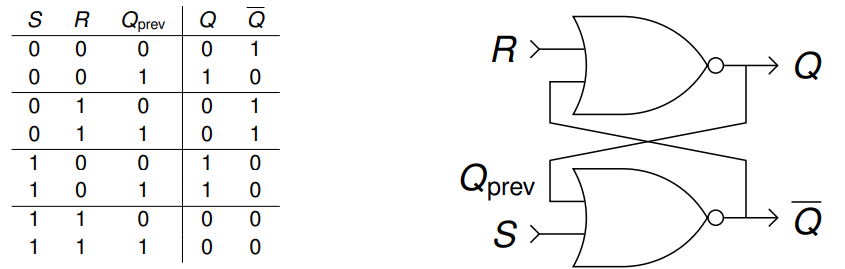
\includegraphics[height=3cm]{srlatch2}
				\end{center}
			\end{figure}
	\end{itemize}
	
\item \textbf{JK-Latch}
	\begin{itemize}
	\item[]		
				\begin{minipage}{0.25\textwidth}
					\begin{figure}[H]
					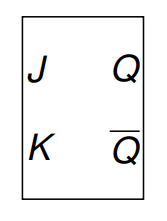
\includegraphics[height=3cm]{jklatch1}
					\end{figure}
				\end{minipage}
				\begin{minipage}[t]{0.6\textwidth}
					\vspace{-1.25cm}
					\begin{itemize}
					\item Ungültigen Zustand SR am SR-Latch verhindern
					\item $\overline{J}~\overline{K} \rightarrow$ Zustand halten
					\item $\overline{J}~K \rightarrow$ Zustand 0 rücksetzen,falls nötig
					\item $J~\overline{K} \rightarrow$ Zustand auf 1 setzen,falls nötig
					\item $J~K \rightarrow$ Zustand invertieren
					\end{itemize}
				\end{minipage}
				
	\item[] \begin{figure}[H]
				\begin{center}
				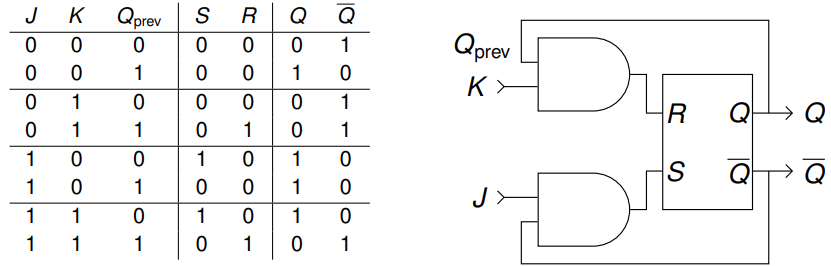
\includegraphics[height=3cm]{jklatch2}
				\end{center}
			\end{figure}
	\end{itemize}
	
\item \textbf{D-Latch}
	\begin{itemize}
	\item[]		
				\begin{minipage}{0.25\textwidth}
					\begin{figure}[H]
					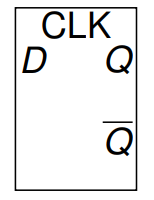
\includegraphics[height=3cm]{dlatch1}
					\end{figure}
				\end{minipage}
				\begin{minipage}[t]{0.6\textwidth}
					\vspace{-1.25cm}
					\begin{itemize}
					\item Daten-Latch mit Taktsignal (CLK) und Dateneingang (D)
					\item CLK = 1 $\rightarrow$ Zustand auf D setzen (Latch transparent)
					\item CLK = 0 $\rightarrow$ Zustand halten (Latch nicht transparent)
					\item ungültiger Zustand am SR-Latch wird vermieden
					\item Rückkopplung nur noch im SR-Latch
					\end{itemize}
				\end{minipage}
				
	\item[] \begin{figure}[H]
				\begin{center}
				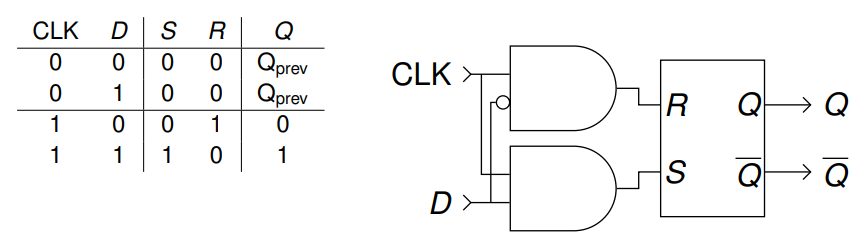
\includegraphics[height=3cm]{dlatch2}
				\end{center}
			\end{figure}
	 
	\item Probleme des D-Latch:
		\begin{itemize}
		\item D-Latch ist taktphasen-gesteuert (Hälfte der Zeit transparent, Hälfte der Zeit kombinatorisch)
		\item breites ''Abtastfenster'' sorgt für Unschärfe
		\item periodische Taktsignale symmetrisch (0-Phase und 1-Phase gleich lang)
		\item[] \begin{figure}[H]
				\begin{center}
				
\includegraphics[height=0.75cm]{dlatch3}
				\end{center}
			\end{figure}
		\end{itemize}
	\end{itemize}

\end{itemize}

\subsection{Flip-Flops}
\begin{itemize}

\item \textbf{D-Flip-Flop}
	\begin{itemize}
	\item[]		
				\begin{minipage}{0.25\textwidth}
					\begin{figure}[H]
					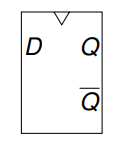
\includegraphics[height=3cm]{dflipflop1}
					\end{figure}
				\end{minipage}
				\begin{minipage}[t]{0.6\textwidth}
					\vspace{-2.25cm}
					\begin{figure}[H]
					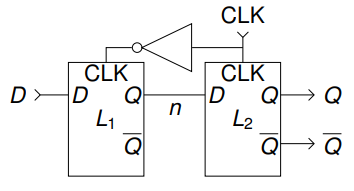
\includegraphics[height=3cm]{dflipflop2}
					\end{figure}
				\end{minipage}
	\end{itemize}
	\begin{itemize}
	\item Zwei D-Latches in Serie ($L_1$ = Master | $L_2$ = Slave | komplementäre Taktsignale)
 	\item CLK = 0:
 		\vspace{-0.3cm}
 		\begin{itemize}
 		\item Master transparent $\rightarrow n = D$
 		\item Slave nicht transparent $\rightarrow$ Q unverändert
 		\end{itemize}
 	\item CLK = 1:
 		\vspace{-0.3cm}
 		\begin{itemize}
 		\item Master nicht transparent $\rightarrow n$ unverändert
 		\item Slave transparent $\rightarrow Q = n$
 		\end{itemize}
 	\item Taktflanken-gesteuert
 		\vspace{-0.3cm}
 		\begin{itemize}
 		\item genau bei steigender CLK Flanke wird $Q=D$
 		\item Übernahme des Wertes von D, der unmittelbar vor der Taktflanke anliegt
 		\end{itemize}
 	\end{itemize}
 	
\item \textbf{Flip-Flops mit Taktfreigabe}
	\begin{itemize}
	\item[]		
				\begin{minipage}{0.25\textwidth}
					\begin{figure}[H]
					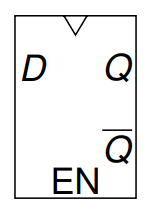
\includegraphics[height=3cm]{takt1}
					\end{figure}
				\end{minipage}
				\begin{minipage}[t]{0.6\textwidth}
					\vspace{-2.25cm}
					\begin{figure}[H]
					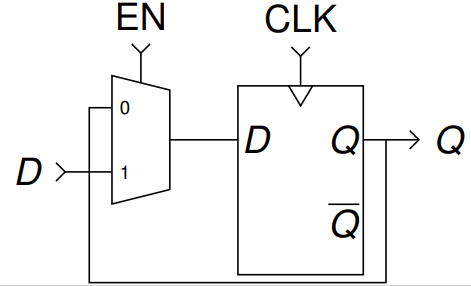
\includegraphics[height=3cm]{takt2}
					\end{figure}
				\end{minipage}
	\end{itemize}
	\begin{itemize}
		\item Freigabeeingang steuert, wann Daten gespeichert werden
		\item $EN = 1 \rightarrow D$ wird bei steigender CLK-Flanke gespeichert
		\item $EN = 0 \rightarrow Q$ bleibt auch bei steigender CLK-Flanke unverändert
 	\end{itemize}
 	
\item \textbf{Zurücksetzbare Flip-Flops}
	\begin{itemize}
	\item[]		
				\begin{minipage}{0.25\textwidth}
					\begin{figure}[H]
					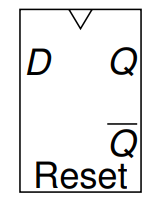
\includegraphics[height=3cm]{reset1}
					\end{figure}
				\end{minipage}
				\begin{minipage}[t]{0.6\textwidth}
					\vspace{-2.25cm}
					\begin{figure}[H]
					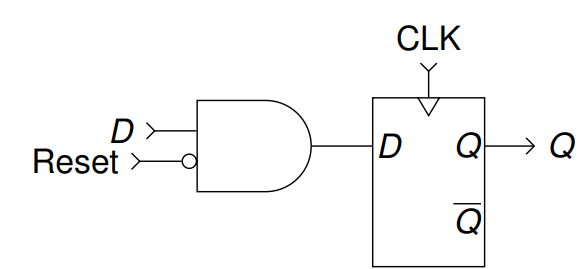
\includegraphics[height=3cm]{reset2}
					\end{figure}
				\end{minipage}
	\end{itemize}
	\begin{itemize}
		\item Reset setzt internen Zustand unabhängig von D auf 0
		\item synchron: nur zur steigenden Taktflanke wirksam
		\item asynchron: jederzeit (unabhängig von CLK)
 	\end{itemize} 
 
\end{itemize}

 
\subsection{Entwurf synchroner Schaltungen}

\begin{itemize}

\item \textbf{Rückkopplungen durch Register aufbrechen}
	\begin{itemize}
	\item halten den Zustand der Schaltung
	\item ändern Zustand nur zur Taktflanke
		\begin{itemize}
		\item[$\rightarrow$] gesamte Schaltung synchronisiert mit Taktflanke
		\end{itemize}
	
	\end{itemize}

\item \textbf{Regeln für Aufbau}
	\begin{itemize}
	\item jedes Schaltungselement ist entweder Register oder kombinatorische Schaltung
	\item mindestens ein Schaltungselement ist ein Register
	\item alle Register werden durch gleiches Taktsignal gesteuert
	\item jeder zyklische Pfad enthält mindestens ein Register
	\item z.B.: Anwendung in endlichen Zustandsautomaten
	\end{itemize}	 


\end{itemize}

\subsection{Endliche Automaten}

\begin{itemize}

\item \textbf{Finite State Machines (FSM)}
	\begin{itemize}
	
	
	\item synchrone sequentielle Schaltungen mit:
		\begin{itemize}
		\item $n$ Eingabebits | $k$ Ausgabebits
		\item ein interner Zustand ($m \geq 1$ Bits) | Takt und Reset
		\end{itemize}
		
	\item in jedem Takt (zur steigenden Flanke):
		\begin{itemize}
		\item Reset aktiv $\rightarrow$ Zustand = Startzustand
		\item Reset inaktiv $\rightarrow$ neuen Zustand/Ausgaben aus aktuellem Zustand/Eingaben 
		\item[] \begin{figure}[H]
				\begin{center}
				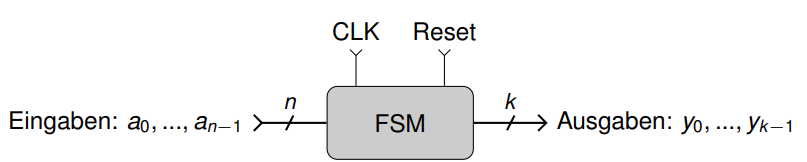
\includegraphics[height=2cm]{fsm1}
				\end{center}
				\end{figure}
		\end{itemize}
	
\item \textbf{FSM als gerichtete Graphen}
	\begin{itemize}
	
	\item  Zustände (States) als Knoten ($S_0,S_1$)
	\item Zustandsübergänge (Transitions) als Kanten
		\begin{itemize}
		\item keine Selbstschleifen
		\item Pfade eindeutig
		\item leere Bedingung entspricht 1
		\end{itemize}
	\item genau eine Kante ohne Startpunkte für Reset
	\item Ausgaben
		\begin{itemize}
		\item An Kanten (Mealy-Automat)
		\item in Zuständen (Moore-Automat)
		\item als boole'scher Ausdruck (Mintern)
		\end{itemize}
	
	\end{itemize}
	
\item \textbf{Zustandsübergangs- und Ausgabetabelle}
	\begin{itemize}
	\item maschinenlesbare Darstellung
	\item kann Don't Cares verwenden
	\item aktueller Zustand $S$ | nächster Zustand $S'$
	\item implizite Bedingungen (Selbstschleifen) beim Ableiten aus Diagrammen beachten
	\end{itemize}
	
\item \textbf{FSM als synchrone sequentielle Schaltung}
	\begin{itemize}
	\item Zustandsregister (Speichern von $S$, Übernahme von $S'$
	\item Zustandsübergangstabelle und Ausgangstabelle mithilfe von kombinatorischer Logik
		\begin{itemize}
		\item[$\rightarrow$] binäre Kodierung der Zustände und Ein-/Ausgaben notwendig
		\end{itemize}
		
	\item[] \begin{figure}[H]
				\begin{center}
				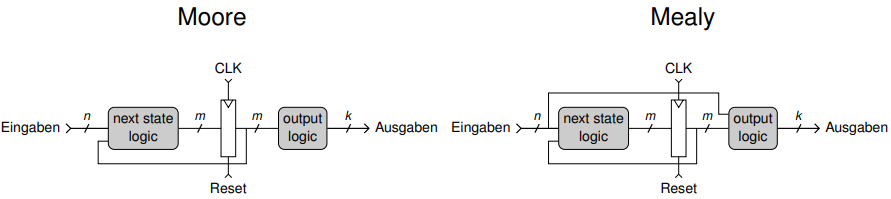
\includegraphics[height=3cm]{fsmsequentiell}
				\end{center}
			\end{figure}
	\end{itemize}
	
\item \textbf{Zustandskodierung $cs: S \rightarrow \mathbb{B}^m$}
	\begin{itemize}
	\item weist jedem Zustand einen m Bit breiten Wert zu
	\item Freie Wahl, z.B. durchnummerieren $cs(S_k)=(s_{m-1}...s_0)$ mit $u_{2,m}(s_{m-1}...s_0)=k$
	\item Effizienz der Kodierung abhängig von Anwendungsfall
	\item Kodierung der Ein-/Ausgänge ist i.d.R. von der Anwendung vorgegeben
	\item Beispiele für Kodierungen und Automaten auf Folien (Foliensatz 8 oder Übungen)
	\end{itemize}


\item \textbf{Entwurfsverfahren}
	\begin{itemize}
	\item Definiere Ein- und Ausgänge
	\item Wähle zwischen Moore- und Mealy-Automat
	\item Zeichne Zustandsdiagramm
	\item Kodiere Zustände (und ggf. Eingänge-/Ausgänge)
	\item Stelle Zustandsübergangstabelle und Ausgabetabelle auf
	\item Stelle boole'sche Gleichungen für Zustandsübergangs und Ausgangslogik mit Don't Cares auf
	\item Entwerfe Schaltplan: Gatter + Register
	\end{itemize}

\item \textbf{Mealy vs Moore}
	\begin{itemize}
	\item muss von Fall zu Fall neu bewertet werden
	\item Moore besser, wenn Ausgaben statisch
	\item Mealy besser, wenn Ausgaben kurzfristige Aktionen auslösen
	\item Mealy reagiert schneller auf Änderungen der Eingabe
	\item Beispiele zur Vrdeutlichung auf den Folien
	\end{itemize}
	
\item \textbf{Zerlegung von Zustandsautomaten}
	\begin{itemize}
	
	\item Aufteilen komplexer FSMs in einfachere interagierende FSMs
	\item zerlegte FSMs kommunizieren untereinander
	\item Ampelbeispiel auf Folien
	
	\end{itemize}

\end{itemize}
\end{itemize}


\subsection{Zeitverhalten}
\begin{itemize}

\item \textbf{Zentrale Fragestellungen}
	\begin{itemize}
	
	\item Flip-Flop übernimmt $D$ zur steigenden Taktflanke
	\item Was passiert bei zeitgleicher Änderung von $D$ und CLK?
	\item Was heißt unmittelbar vor der Taktflanke?
	\item Wie schnell wird neuer Zustand am Ausgang sichtbar?
	\item Was muss beachtet werden?
	\item[] \begin{figure}[H]
				\begin{center}
				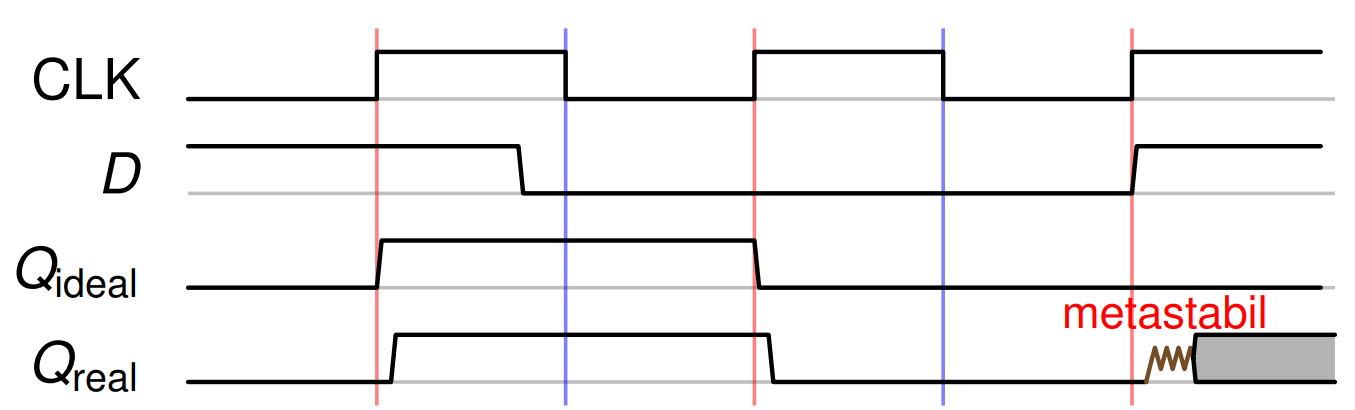
\includegraphics[height=3cm]{zeitseq1}
				\end{center}
			\end{figure}
	
	
	\end{itemize}
	
\pagebreak	
	
\item \textbf{Metastabilität}
	\begin{itemize}
	\item zeitlich begrenzter und undefinierter Zustand
	\item geht nach zufälliger Verzögerung in einen stabilen Zustand über
	\end{itemize}
	
\item \textbf{Zeitanforderungen an DFF Eingangssignal}
	\begin{itemize}
	\item Dateneingang $D$ muss vor und nach dem Abtasten stabil sein
		\begin{itemize}
		\item[$\rightarrow$] Vermeidung von Metastabilität
		\end{itemize}
	
	\item $t_{setup}$: Zeitintervall vor Taktflanke, in dem $D$ stabil sein muss
	\item $t_{hold}$: Zeitintervall nach Taktflanke, in dem $D$ stabil sein muss
	\item $t_a$: Abtastzeitfenster : $t_{setup}+t_{hold}$ (''aperture time'')
	\item[] \begin{figure}[H]
				\begin{center}
				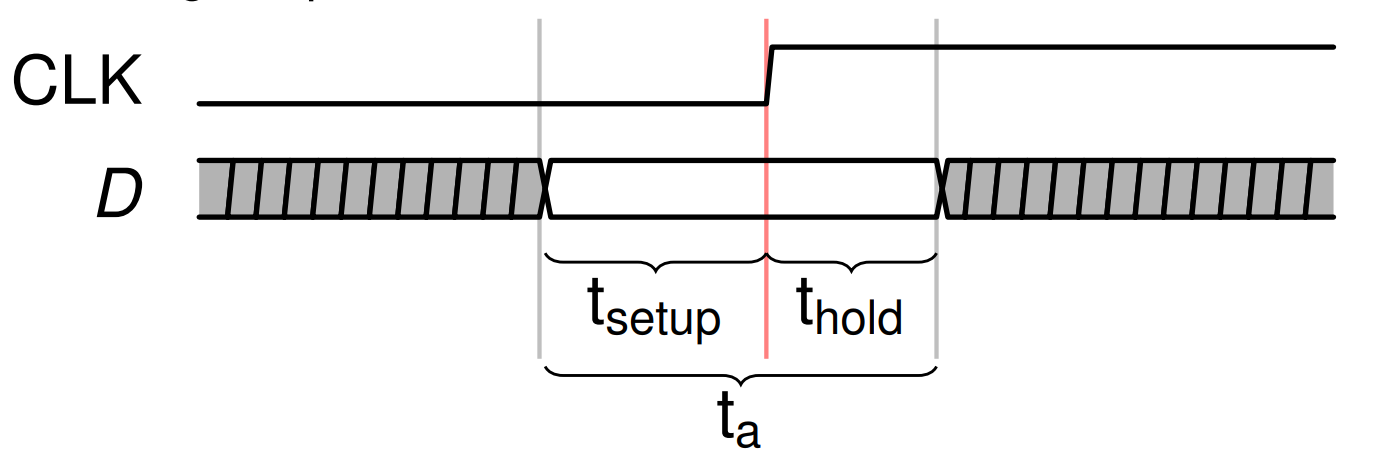
\includegraphics[height=2.5cm]{dff1}
				\end{center}
			\end{figure}
	\end{itemize}
	
\item \textbf{Zeitcharakteristik des DFF Ausgangssignals}
	\begin{itemize}
	\item Verzögerung des Registerausgangs relativ zur steigenden Taktflanke
	\item Kontaminationsverzögerung ($t_{ccq}$): kürzeste Zeit bis Q umschaltet
	\item[] (''contamination delay clock-to-Q'')
	\item Laufzeitverzögerung ($t_{pcq}$): längste Zeit bis Q sich stabilisiert
	\item[] (''propagation delay clock-to-Q'')\\
	\item[] \begin{figure}[H]
				\begin{center}
				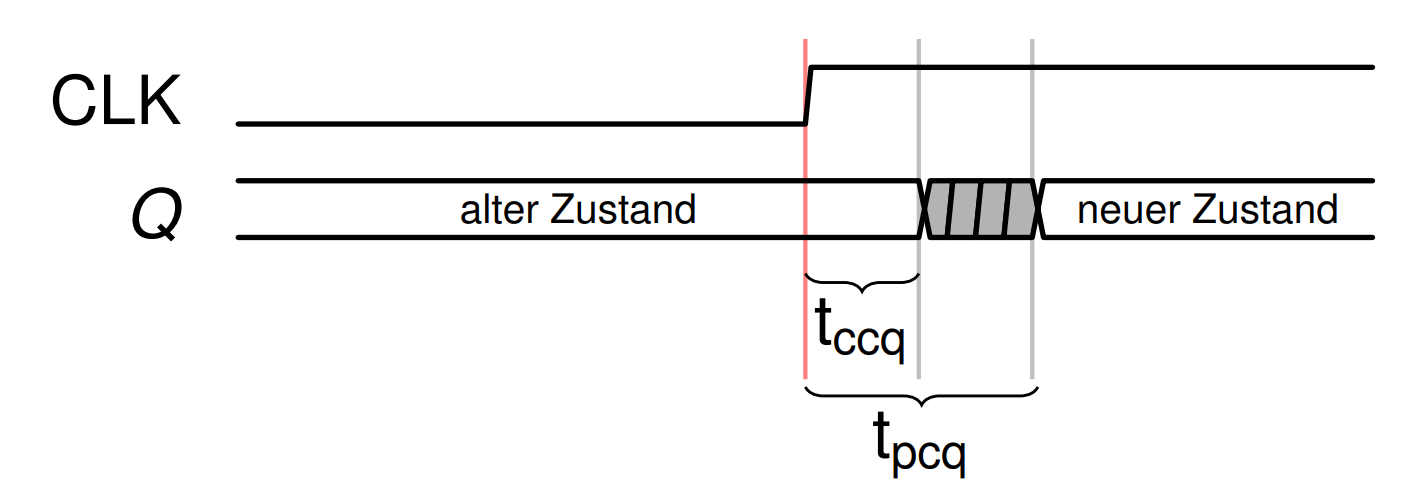
\includegraphics[height=2.5cm]{dff2}
				\end{center}
			\end{figure}
	\end{itemize}

\item \textbf{Dynamische Entwurfsdisziplin}
	\begin{itemize}
	\item[]		
				\begin{minipage}{0.25\textwidth}
					\begin{figure}[H]
					\includegraphics[height=5cm]{entwurfsdisziplin}
					\end{figure}
				\end{minipage}
				\begin{minipage}[t]{0.65\textwidth}
					\vspace{-2.25cm}
					\begin{itemize}
					\item $D_2$ abhängig von Verzögerungen des ersten Registers + Gatter
					\item Timing Bedingungen des zweiten Registers müssen erfüllt sein:
						\begin{itemize}
						\item[$\rightarrow$] $t_{ccq,1}+t_{cd} \geq t_{hold,2}$
						\item[$\rightarrow$] $t_{pcq,1}+t_{pd} + t_{setup,2} \leq t_{CLK}$
						\end{itemize}
					
					\item Maximale Taktrate wird durch kritischen Pfad bestimmt
						\begin{itemize}
						\item[$\rightarrow$] $f_{CLK}=\frac{1}{t_{CLK}} \leq \frac{1}{t_{pcq}+t_{pd}+t_{setup}}$
						\end{itemize}
					\item Falls Hold-Bedingung verletzt: 
						\begin{itemize}
						\item[$\rightarrow$] Einfügen von Buffern auf kürzestem Pfad
						\end{itemize}
					\end{itemize}
				\end{minipage}
	\end{itemize}
	
\pagebreak	
	
\item \textbf{Taktverschiebung}
	\begin{itemize}
	\item Takt kommt nicht bei allen Registern gleichzeitig an (Chip-Unterschiede,..)
	\item $t_{skew}$ ist maximale Differenz der Taktankunftszeit zwischen zei Registern
	\item[] \begin{figure}[H]
				\begin{center}
				\includegraphics[height=2.5cm]{tskew}
				\end{center}
			\end{figure}
	\end{itemize}
	
\item \textbf{Timing-Bedingunge mit Takt-Verschiebung}
	\begin{itemize}
	\item Bedingungen müssen auch im Worst-Case eingehalten werden
		\begin{itemize}
		\item[$\rightarrow$] $t_{ccq,1}+t_{cd} \geq t_{hold,2} + t_{skew}$
		\item[$\rightarrow$] $t_{pcq,1}+t_{pd} + t_{setup,2} + t_{skew} \leq t_{CLK}$
		\end{itemize}
	
	\item Timing wird dadurch meist enger
	\end{itemize}
	
\item \textbf{Verletzung der dynamischen Entwurfsdisziplin}
	\begin{itemize}
	\item[]		
				\begin{minipage}{0.25\textwidth}
					\begin{figure}[H]
					\includegraphics[height=2cm]{verletzungdyn}
					\end{figure}
				\end{minipage}
				\begin{minipage}[t]{0.65\textwidth}
					\vspace{-1.5cm}
					\begin{itemize}
					\item asynchrone Eingänge 
					\item[$\Rightarrow$]Eventuelle Nichteinhaltung der Timing-Bedingungen
					\item Schieberegister für Synchronisation
					\item erstes Flip-Flop kann metastabil werden
					\item kippt i.d.R. vor nächster Taktflanke in stabilen Zustand
					\item[$\Rightarrow$] zweites Flip-Flop wird nicht metastabil
					\end{itemize}
				\end{minipage}
	

	\end{itemize}
	
\end{itemize}


\subsection{Parallelität}
\begin{itemize}

\item \textbf{Arten der Parallelität}
	\begin{itemize}
	\item räumliche Parallelität:
		\begin{itemize}
		\item[$\rightarrow$] mehrere Aufgaben durch vervielfachte Hardware gleichzeitig bearbeiten
		\end{itemize}
	
	\item zeitliche Parallelität:
		\begin{itemize}
		\item[$\rightarrow$] Aufgaben in mehrere Unteraufgaben aufteilen
		\item[$\rightarrow$] Unteraufgaben parallel ausführen
		\end{itemize}
	
	\end{itemize}
	
\item \textbf{Begriffe}
	\begin{itemize}
	\item Datensatz: Vektor aus Eingabewerten $\rightarrow$ Vektor aus Ausgabewerten
	\item Latenz: Zeit von Eingabe des Datensatzes bis zur Ausgabe des Ergebnisses
	\item Durchsatz: Anzahl von Durchsätzen pro Zeiteinheit
		\begin{itemize}
		\item[$\rightarrow$] Parallelität erhöht Durchsatz
		\end{itemize}
	
	\end{itemize}
	
\item \textbf{Pipelining}
	\begin{itemize}
	\item Pipelinestufen sollten möglichst lang sein
		\begin{itemize}
		\item[$\rightarrow$] längste Stufe bestimmt maximale Taktfrequenz $f_{CLK}$
		\item[$\rightarrow$] Latenz = Pipelinestufen * Taktfrequenz
		\end{itemize}			
	\item mehr Pipelinestufen:
		\begin{itemize}
		\item[$\rightarrow$] höherer Durchsatz, da höhere Taktfrequenz
		\item[$\rightarrow$] aber auch höhere Latenz
		\item[$\rightarrow$] lohnt sich nur bei vielen Datensätzen
		\end{itemize}
		
	\end{itemize}

\end{itemize}

%--------------------------------------------------------------------------------

\section{Hardware-Beschreibungssprachen}


\subsection{Allgemein}
\begin{itemize}

\item \textbf{Notwendigkeit und Anwendung}
	\begin{itemize}
	\item verständliche und einheitliche Beschreibungssprache
	\item Benötigt, um steigende Komplexität zu beherrschen
	\item Aktuelle Tendenz zu höheren Abstraktionsleveln bei der Entwicklung
	\end{itemize}
	
\item \textbf{Von HDL zu Logikgattern}
	\begin{itemize}
	\item $Simulation$ des Verhaltens der beschriebenen Schaltung (Fehlersuche einfacher als in realer Schaltung)
	\item $Synthese$ übersetzt Hardware-Beschreibungen in Netzliste
	\item $Netzliste$ beschreibt die Schaltungselemente und Verbindungsknoten
	\end{itemize}
\end{itemize}

\subsection{Kombinatorische Logik (Einführung)}
\begin{itemize}

\item \textbf{SystemVerilog Module}
	\begin{itemize}
	\item Modul beschreibt, wie eine Aufgabe durchgeführt wird
	\item Schnittstellenbeschreibung mithilfe von Eingängen, Ausgängen und Parameter
	\item zwei Arten der Beschreibung
	\begin{itemize}
	\item[$\rightarrow$] Struktur (Wie ist die Schaltung aus Modulen aufgebaut?)
		\item[$\rightarrow$] Verhalten (Was tut die Schaltung?)
	\end{itemize}
		
	\end{itemize}
	
\item \textbf{Modulbeschreibung}
	\begin{itemize}
	\item Befehle auf Hilfsblatt
	\item $\sim$ NOT   \& AND   | OR
	\end{itemize}
	
\item \textbf{Syntax}
	\begin{itemize}
	\item Case-Sensitive
	\item Bezeichner dürfen nicht mit Ziffern anfangen
	\item Anzahl von blank space irrelevant
	\item Kommentare wie in Java (// und /*...*/)
	\end{itemize}

\end{itemize}

\subsection{Modulhierarchie}
\begin{itemize}
\item \textbf{Modulinstanzierung: (innerhalb eines anderen Moduls)}
	\begin{itemize}
	
	\item[]
		\begin{lstlisting}
		module and3 (input logic a, b, c, output logic y);
			assign y = a & b & c;
		endmodule
		\end{lstlisting}		
	\item[]	
		\begin{lstlisting}
		module inv (input logic a, output logic y);
			assign y = ~a;
		endmodule
		\end{lstlisting}		
	\item[]
		\begin{lstlisting}
		module nand3 (input logic d, e, f, output logic w);
			logic s; 							//Internes Signal zur Verbindung
			and3 andgate(d, e, f, s);  			//Instanz von and3 namens andgate
			inv inverter(s, w);				
		endmodule
		\end{lstlisting}	
	\end{itemize}
	
\pagebreak	
	
\item \textbf{Portzuweisung nach Position oder Namen}
	\begin{itemize}
	\item[]
		\begin{lstlisting}
		module nand3_named (input logic d, e, f, output logic w);
			logic s;
			and3 andgate(.a(d), .b(e), .c(f), .y(s));
			inv inverter(.a(s), .y(w)); 	
		endmodule
		\end{lstlisting}
	\item 10-100 Ports pro Modul nicht unüblich
		\begin{itemize}
		\item[$\rightarrow$] absolute Portzuweisung per Namen übersichtlicher	
		\end{itemize}
		
	
	\end{itemize}
	
\item \textbf{Bitweise Verknüpfungsoperatoren}
	\begin{itemize}
	
	\item[] 
		\begin{lstlisting}
		module gates (input logic [3:0] a, b,
					  output logic [3:0] y1, y2, y3, y4, y5);
			assign y1 = a & b; // AND
			assign y2 = a | b; // OR
			assign y3 = a ^ b; // XOR
			assign y4 = ~(a & b); // NAND
			assign y5 = ~(a | b); // NOR
		endmodule		
		
		\end{lstlisting}	
		
	\item [3:0] $\rightarrow$ Bitbreite = 4

	\end{itemize}
	
\item \textbf{Reduktionsoperationen(unär)}
	\begin{itemize}
	
	\item[]
		\begin{lstlisting}
		module and8 (input logic [7:0] a, output logic y);
			assign y = &a; // assign y = a[7] & a[6] & ... & a[0];
		endmodule	
		\end{lstlisting}	
		
	\item Weitere Operationen: | (OR)   $\wedge$ (XOR)   $\sim$| (NOR)   $\sim$\& (NAND)   $\sim\wedge$ (XNOR)
	
	\end{itemize}
	
\item \textbf{Bedingte Zuweisung}
	\begin{itemize}
	\item $y = s ~ ? ~ d1~:~d0;$
	\item Falls s = 1, dann y = d1, sonst y = d0
	\end{itemize}

\item \textbf{Interne Verbindungsknoten}
	\begin{itemize}
	\item[]
		\begin{lstlisting}
		module fulladder (input logic a, b, cin, output logic s, count);
			logic p, g; //interne Verbindungsknoten
			assign p = a ^ b;
			assign g = a & b;
			assign s = p ^ cin;
			assign cout = g | (g & cin);
		endmodule
		\end{lstlisting}
		
	\item[] \begin{figure}[H]
				\begin{center}
				\includegraphics[height=2cm]{verbindungsknoten}
				\end{center}
			\end{figure}
	\end{itemize}
	
\item \textbf{Syntax für numerische Literale}
	\begin{itemize}
	\item <N>'<B><wert>
	\item Bitbreite N, Basis B (d,b,o,h) (default: 32'd)
	\item Unterstriche als optische Trenner möglich
	\item Beispiele:
		\begin{itemize}
		\item 8'b11 $\Rightarrow 0000~0011$
		\item 3'd6 $\Rightarrow 110$
		\item 42 $\Rightarrow 0000...0101010$
		\end{itemize}
	\end{itemize}

\item \textbf{Konkatenation}
	\begin{itemize}
	
	\item[]
		\begin{lstlisting}
		module concat (input logic [2:0] a, b, output logic [11:0] y);
			assign y = {a[2:1], {3{b[0]}}, a[0], 6'b100010};
			// y = a[2] a[1] b[0] b[0] b[0] a[0] 1 0 0 0 1 0;
		endmodule		
		\end{lstlisting}
	
	\end{itemize}
	
\item \textbf{Hochohmiger Ausgang Z}
	\begin{itemize}
	\item Z darf nur an Ausgängen verwendet werden
	\item für interne Signale aber simulierbar
	\end{itemize}

\item \textbf{Verzögerung: \#Zeiteinheiten}
	\begin{itemize}
	\item Festlegen der Verzögerung vor Modul: 
		\begin{itemize}
		\item[$\rightarrow$]'timescale 1ns / 10 ps (Zeiteinheit / Präzision für Rundung)
		\end{itemize}
	\item nach assign \#n für Verzögerung um n Zeiteinheiten
	\end{itemize}

\end{itemize}

\subsection{Datentypen}
\begin{itemize}

\item \textbf{Auswahl wichtiger Datentypen}
	\begin{itemize}
	\item bit = {1'b0, 1'b1} (zweiwertige Logik)
	\item logic = {1'b0, 1'b1, 1'bx, 1'by} (vierwertige Logik)
	\item int = {-2**31,...,2**31-1} = bit signed [31:0]
	\item integer = {-2**31,...,2**31-1} = logic signed [31:0]
	\item enum = Aufzählung symbolischer Werte
	\item Vektoren und Arrays
	\end{itemize}
	
\item \textbf{Vektoren und Arrays}
	\begin{itemize}
	\item Allgemein:
	\item[]
		\begin{lstlisting}
		// Deklaration
		logic [7:0] bitVector = 8'hAB; // 8 Bit Vektor, jedes Element 8'hAB [MSB:LSB]
		logic 		bitArray [0:7] 		// 8 Bit Array [first:last]
		
		
		// Zugriffe / Modifikationen
		initial begin 
			#1 bitVector  		= 8'hCD; // alle Vektorenbits ueberschreiben
			#1 bitVector[5] 	= 1'b1;	 // Vektorbits einzeln ueberschreiben
			#1 bitVector[3:0]	= 4'hF;	 // Vektorbereich ueberschreiben
			
			// Array-Zugriff nur elementweise moeglich
			for (int i = 0; i <$size(bitArray); i++} #1 bitArray[i] = bitVector[i];
		end
		
		\end{lstlisting}
		
\pagebreak		
		
	\item Operationen auf Vektoren
	\item[]
		\begin{lstlisting}
		
		module vecop (input logic [3:0] A, input logic [3:0] B,
						output logic U, V, output logic [3:0] W,
						output logic [1:0] X, output logic [5:0] Y,
						output logic [7:0] Z);
			
			// Reduktion
			assign U = & A; 		// U = A[0] & A[1] & A[2] & A[3]
			
			// logische Verknuepfung
			assign V = A && B 		// V = (A[0] | A[1] |...) & (B[0] | B[1] |...)
			
			// bitweise Verknuepfung 
			assign W = A & B // W[0] = (A[0] & B[0]),...
			
			// Konkatenation
			assign {X,Y} = {A,B}; // X = A[3:2], Y[5:4] = A[1:0], Y[3:0] = B
			
			// (unsigned) Arithmetrik
			assign Z = A * B;
			
		\end{lstlisting}
		
	\item Einschränkungen auf Arrays
		\begin{itemize}
		\item nicht als Ports verwendbar
		\item nicht mit assign verwendbar (kein Part Select (nur einzelne Elemente), keine Zuweisung ganzer Arrays)
		\item keine Reduktion/Konkatenation
		\item keine bitweisen/logischen/arithmetischen Operationen
		\end{itemize}
		
	\item Speicher als Vektor Arrays
	\item[]
	\begin{lstlisting}
	//			 Breite 			Tiefe
	logic [3:0] mem [0:15]; // 16 Worte zu je 4 Bit
	
	initial begin 
			for (int i = 0; i <$size(mem); i++) #1 mem[i] = i; 
			
			// Zugriff auf Bits in Vektor-Array
			mem[0][3] = ~mem[0][3];
	end
	\end{lstlisting}
	\end{itemize}

\end{itemize}



\subsection{Modellierung kombinatorischer Schaltungen}
\begin{itemize}

\item \textbf{assign Statement}
	\begin{itemize}
	\item[]
		\begin{lstlisting}
		module example (input logic a, b, c, output logic y);
			assign y = ~a & ~b & ~c | a & ~b & ~c | a & ~b & c;
		endmodule
		\end{lstlisting}
	\item auch continuous assignment genannt
	\item Linke Seite (LHS, left hand side): Variable oder Port
	\item Rechte Seite (RHS, right hand side): logischer Ausdruck
	\item Zuweisung, wenn sich der Wert von RHS ändert
	\end{itemize}
	
\item \textbf{always-comb Block}
	\begin{itemize}
	\item always\_comb <instruction>
		\begin{itemize}
		\item[$\rightarrow$] zum Zeitpunkt 0, nachdem alle initial und always Blöcke gestartet sind
		\item[$\rightarrow$] wenn sich der Wert von RHS ändert
		\end{itemize}
		
	\item LHS Variablen dürfen nicht von anderen Blöcken geschrieben werden
	\end{itemize}

\pagebreak

\item \textbf{Fallunterscheidungen (case)}
	\begin{itemize}
	\item[]
		\begin{lstlisting}
		module sevenseg (input logic [3:0] A, output logic [6:0] S);
			always_comb case (A)
					0: S = 7'b011_1111;
					1: S = 7'b000_0110;
					...
			  default: 	S = 7'b000_0000;
			endcase
		endmodule
		\end{lstlisting}
		
	\item case darf nur in always/always\_comb Blöcken verwendet werden
	\item Alle Eingabeoptionen abdecken (explizit oder über default)
	\end{itemize}

\item \textbf{Fallunterscheidungen (casez)}
	\begin{itemize}
	\item[]
		\begin{lstlisting}
		module priority_encoder (input logic [3:0] A, output logic [3:0] Y);
			always_comb casez(A) //casez erlaubt Don't cares als ?
					4'b1???: Y = 4'b1000;
					4'b01??: Y = 4'b0100;
					4'b001?: Y = 4'b0010;
					4'b0001: Y = 4'b0001;
					default: Y = 4'b0000;
			endcase
		endmodule
		\end{lstlisting}
	\end{itemize}

\item \textbf{Eigenschaften von assign und always\_comb}
	\begin{itemize}
	\item werden immer ausgeführt, wenn sich ein Signal auf der rechten Seite ändert
		\begin{itemize}
		\item[$\rightarrow$] Eigenes Sprachkonstrukt für sequentielle Logik aufgrund interner Zustände
		\end{itemize}
		
	\item Reihenfolge im Quellcode nicht relevant
		\begin{itemize}
		\item[$\rightarrow$] Blockierende Signalzuweisungen (a = b) innerhalb von Blöcken (begin/end) seriell ausgeführt
		\end{itemize}
	\end{itemize}

\end{itemize}


\subsection{Modellierung sequentieller Schaltungen}
\begin{itemize}

\item \textbf{Grundkonzept von always-Blöcken}
	\begin{itemize}
	\item führt eine Instruktion als Endlosschleife aus
	\item durch Klammerung (begin...end) werden Instruktionen zusammengefasst
	\item alle always-Blöcke werden parallel ausgeführt
	\item ohne explizite Verzögerungsangaben (\#n) wird die simulierte Zeit durch Ausführung nicht erhöht
	\item[]
		\begin{lstlisting}
		logic a;
		always begin
			a = 1;
			#1;
			a = 0;
			#2;
		end
		
		logic b = 0;
		always #0.5 b = !b;
		\end{lstlisting}
	\end{itemize}
	
\pagebreak	
	
\item \textbf{Interpretation von Verzögerungszeiten}
	\begin{itemize}
	\item 'timescale <base> / <precision> 	(vor Modul spezifiziert)
	\item <base> wird mit angegebenem <tval> multipliziert
	\item Auch arithmetische Ausdrücke für <tval>
	\item[]
		\begin{lstlisting}
		'timescale 1 ns / 10 ps
		
		module delay;
			logic c = 0;
			always #(1/3.0) c = !c; // 0.33ns
			
			logic [3:0] d = 0;
			always #(d + 1) d = d + 1;
		endmodule				
		\end{lstlisting}
	
	
	\end{itemize}
	
\item \textbf{Warten auf Ereignisse}
	\begin{itemize}
		
	\item @ <expr> wartet auf Änderung von kombinatorischen Ausdruck <expr>
	\item @ (posedge <expr>) wartet auf steigende Flanke von <expr> (0 $\rightarrow$ 1, 0 $\rightarrow$ x,..)
	\item @ (nededge <expr>) wartet auf fallende Flanke von <expr> (1 $\rightarrow$ 0, 1 $\rightarrow$ x,..)
	\item @ (<event1> or <event2>) wartet auf das Eintreten eines der aufgelisteten Ereignisse
		\begin{itemize}
		\item[$\rightarrow$] or kann auch durch , ersetzt werden
		\item[$\rightarrow$] wird auch als Sensitivitätsliste bezeichnet
		\end{itemize}
	\item @* wartet auf Änderung eines der im always Block gelesenen Signale
	\item Warte-Statements können an beliebiger Stelle im always Block stehen
	
	\end{itemize}
	
\item \textbf{Zuweisungssequenzen in always-Blöcken}
	\begin{itemize}
	\item blockierende Zuweisungen: <signal> = <expr>;
		\begin{itemize}
		\item[$\rightarrow$] <expr> wird ausgewertet und an <signal> überweisen, bevor nächste Zuweisung behandelt wird
		\item[$\rightarrow$] blockierende Zuweisungen werden sequentiell behandelt
		\end{itemize}
	\item Nicht-blockierende Zuweisungen: <signal> <= <expr>;
		\begin{itemize}
		\item[$\rightarrow$] <expr> wird zwar ausgewertet, aber noch nicht an <signal> überwiesen
		\item[$\rightarrow$] Zuweisung an <signal> erfolgt erst bei Fortschreiten der Systemzeit (\# oder @)
		\item[$\rightarrow$] nicht-blockierende Zuweisungen werden parallel bearbeitet
		\end{itemize}
	\end{itemize}

\item \textbf{Einmalige und kombinatorische Ausführung}
	\begin{itemize}
	\item initial <instruction>
		\begin{itemize}
		\item[$\rightarrow$] entspricht always begin <instruction> @(0); end
		\item[$\rightarrow$] für Initialisierung in der Simulation verwenden
		\end{itemize}
	\item always\_comb <instruction> 
		\begin{itemize}
		\item[$\rightarrow$] verbessert always @* <instruction>
 		\item[$\rightarrow$] einmalige Ausführung zu Beginn der Simulation, auch ohne Änderung der Eingabesignale
 		\item[$\rightarrow$] für komplexe, kombinatorische Logik (for, if/else, case, casez) verwenden
		\end{itemize}
	\end{itemize}

\pagebreak

\item \textbf{Modellierung von Speichelementen}
	\begin{itemize}
	
	\item D-Latch
		\begin{itemize}
		\item[]
			\begin{lstlisting}
			module latch (input logic CLK, D, output logic Q);
				always_latch if (CLK) Q <= D;
			endmodule			
			\end{lstlisting}
		\item always\_latch <instruction>
			\begin{itemize}
			\item[$\rightarrow$] für Schaltungen mit Latches
			\item[$\rightarrow$] entspricht always\_comb <instruction>
			\item[$\rightarrow$] Latches werden kaum benutzt, entstehen meist durch Fehler
			\end{itemize}
		\end{itemize}
	
	\item D-Flip-Flop
		\begin{itemize}
		
		\item[] 
			\begin{lstlisting}
			module dff (intput logic CLK, D, output logic Q);
				always_ff @(posedge CLK) Q <= D;
			endmodule
			\end{lstlisting}	
		
		\item always\_ff <instruction>
			\begin{itemize}
			\item für Schaltungen mit Flip-Flops
			\item entspricht always <instruction>
			\item vergleichbare Verbesserungen wie bei always\_comb
			\end{itemize}				
		
		\end{itemize}		
		
	\item Asynchron rücksetzbarer D-Flip-Flop
		\begin{itemize}
		\item[]
			\begin{lstlisting}
			module dffar (input logic CLK, RST, D, output logic Q);
				always_ff @(posedge CLK, posedge RST)
					if (RST) Q <= 0;
					else 	 Q <= D;
			endmodule
			\end{lstlisting}
		\end{itemize}		
		
	\item Synchron rücksetzbarer D-Flip-Flop
		\begin{itemize}
		\item[]
			\begin{lstlisting}
			module dffr (input logic CLK, RST, D, output logic Q);
				always_ff @(posedge CLK)
					if (RST) Q <= 0;
					else 	 Q <= D;
			endmodule
			\end{lstlisting}
		\end{itemize}			
	
	\item D-Flip-Flop mit Taktfreigabe
		\begin{itemize}
		\item[]
			\begin{lstlisting}
			module dffe (input logic CLK, RST, EN, D, output logic Q);
				always_ff @(posedge CLK)
					if		 (RST) Q <= D;
					else if  (EN) Q <= D;
			endmodule
			\end{lstlisting}
		\end{itemize}			
	
	\end{itemize}
	
\item \textbf{Allgemeine Regeln für Signalzuweisungen (synchrone sequentielle Schaltungen)}
	\begin{itemize}
	\item interne Zustände
		\begin{itemize}
		\item[$\rightarrow$] innerhalb von always\_ff @(posedge CLK)
		\item[$\rightarrow$] mit nicht-blockierenden Zuweisungen (<=)
		\item[$\rightarrow$] möglichst ein/wenige Zustände pro always\_ff Block
		\end{itemize}
	\item einfache kombinatorische Logik durch nebenläufige Zuweisungen (assign)
	\item komplexere kombinatorische Logik
		\begin{itemize}
		\item[$\rightarrow$] innerhalb von always\_comb
		\item[$\rightarrow$] mit blockierenden Zuweisungen (=)
		\end{itemize}		
	\item ein Signal darf NICHT
		\begin{itemize}
		\item[$\rightarrow$] von mehreren nebenläufigen Prozessen (assign/always) beschrieben werden
		\item[$\rightarrow$] innerhalb eines always-Blocks mit block. \& nicht-block. Zuweisungen beschrieben werden
		\end{itemize}
			
	\end{itemize}

\end{itemize}

\subsection{Parametrisierte Module}
\begin{itemize}

\item \textbf{Parametrisierte Module}
	\begin{itemize}
	\item Definieren von Parametern durch Modulschnittstelle
	\item parametrisierte Eigenschaften werden bei Instanziierung durch konkrete Werte ersetzt
	\item Vergleichbar mit Java-Generics
	\item Typische Parameter: Port-Breite, Speichertiefe, Anzahl der Submodule,..
	\item[]
		\begin{lstlisting}
		module register #(parameter WIDTH = 8, parameter DEPTH = 32) (input logic...)
		\end{lstlisting}
	\end{itemize}

\end{itemize}


\subsection{Testrahmen}
\begin{itemize}

\item \textbf{Testumgebungen (testbenches}
	\begin{itemize}
	\item HDL-Programm zum Testen eines HDL-Moduls
	\item getestes Modul (Device under test DUT, Unit under test UUT)
	\item Arten von Testrahmen:
		\begin{itemize}
		\item[$\rightarrow$] einfach: Testdaten an UUT anlegen und Ausgaben anzeigen
		\item[$\rightarrow$] selbstprüfend: Ausgaben zusätzlich auf Korrektheit prüfen
		\item[$\rightarrow$] selbstprüfend mit Testvektoren: variable Testdaten (z.B. aus Datei)
		\end{itemize}
	\end{itemize}
	
\item \textbf{Einfacher Testrahmen}
	\begin{itemize}
	\item[]
		\begin{lstlisting}
		module simble_tb;
			logic a, b, c, y;
			simple uut(a, b, c, y);
			
			initial begin
				//dump changes of all variables to this file
				$dumpfile("simple_tb.vcd");
				$dumpvars;
				
				a = 0; b = 0; c = 0; #10;
							  c = 1; #10;
					   b = 1; c = 0; #10;
					   	      c = 1; #10;
					   	      
				$display("FINISHED simple_tb"); // Textausgabe
				$finish; 						// beendet Simulation
			end
		endmodule
		\end{lstlisting}
	\end{itemize}
	
\item \textbf{Selbstprüfender Testrahmen}
	\begin{itemize}
	\item[]
		\begin{lstlisting}
		module simble_tb2;
			logic a, b, c, y;
			simple uut(a, b, c, y);
			
			initial begin
				//dump changes of all variables to this file
				$dumpfile("simple_tb2.vcd");
				$dumpvars;
				
				a = 0; b = 0; c = 0; #10; assert (y = = = 1) else $error("000 failed.");
							  c = 1; #10; assert (y = = = 0) else $error("001 failed.");
					   b = 1; c = 0; #10; assert (y = = = 0) else $error("010 failed.");
					   	      c = 1; #10; assert (y = = = 0) else $error("011 failed.");
					   	      
				$display("FINISHED simple_tb"); // Textausgabe
				$finish; 						// beendet Simulation
			end
		endmodule
		\end{lstlisting}
	\end{itemize}
	
\item \textbf{Vorhergehensweise}
	\begin{itemize}
	\item Modul ohne Ports
	\item Stimuli erzeugen (Takt, Reset, Eingabedaten)
	\item ''unit under test'' instanziieren
	\item Ausgabedaten und Timing spezifizieren (erschöpfend/zufällig, Grenzfälle bedenken)
	\item wird nicht synthetisiert
	\end{itemize}

\item \textbf{Ausgabe von Statusmeldungen}
	\begin{itemize}
	\item \$display(<format>, <values>*);
	\item Platzhalter:
		\begin{itemize}
		\item[$\rightarrow$] \%d \%b \%h für dezimal, binär und hexadezimal
		\item[$\rightarrow$] \%m für Modulname
		\item[$\rightarrow$] \%t für Zeit (mit Einheit)
		\end{itemize}
	\item \$timeformat(-9, 1, ''ns'', 8); zum Erstellen des Zeitformats
		\begin{itemize}
		\item[$\rightarrow$] Skalierung auf $10^{-9}$ | Eine Nachkommastelle
		\item[$\rightarrow$] ''ns'' als Einheiten-Suffix | 8 anzuzeigende Zeichen
		\end{itemize}
	\end{itemize}

\item \textbf{Auslesen der Simulationszeit}
	\begin{itemize}
	\item \$time: aktuelle Systemzeit als ganze Zahl (int)
	\item \$realtime: aktuelle Systemzeit als rationale Zahl (real)
	\item Zeitspanne zwischen zwei Signalflanken bestimmen:
	\item[]
		\begin{lstlisting}
		'timescale 1 ns / 10 ps
		module deltat;
			logic a = 0; always #3 a <= ~a;
			logic b = 0; always #2 b <= ~b;
			
			real aEvent; always @a aEvent <= $realtime;
			real delay;  always @b delay  <= $realtime - aEvent;
		endmodule
		\end{lstlisting}
	\end{itemize}

\end{itemize}

\subsection{Modellierung endlicher Automaten}
\begin{itemize}
\item \textbf{Grundidee für FSM-Modellierung}
	\begin{itemize}
	\item Logikvektor oder enum für Zustände
	\item rücksetzbare Flip-Flops als Zustandsspeicher
	\item kombinatorische next-state Logik durch case in always\_comb Block
	\item kombinatorische Ausgabe-Logik durch nebenläufige Zuweisungen	
	
	\end{itemize}
	
\item \textbf{Moore Automat für 1101 Mustererkennung}
	\begin{itemize}
	\item[]
		\begin{lstlisting}
		module moore (input logic CLK, RST, A, output logic Y);
			typedef enum logic [2:0] {S0, S1, S2, S3, S4} statetype;
			statetype state, nextstate;
			always_ff @(posedge CLK) state <= RST ? S0 : nextstate;
			
			// next state logic
			always_comb case (state)
				S0: 	 nextstate = A ? S1 : S0;
				S1:		 nextstate = A ? S2 : S0;
				S2: 	 nextstate = A ? S2 : S3;
				S3: 	 nextstate = A ? S4 : S0;
				S4: 	 nextstate = A ? S2 : S0;
				default: nextstate = S0;
			endcase
			
			//output logic
			assign Y = (state = = S4);
		endmodule
				
		\end{lstlisting}
	\end{itemize}
	
\item \textbf{Mealy Automat für 1101 Mustererkennung}
	\begin{itemize}
	\item[]
		\begin{lstlisting}
		module moore (input logic CLK, RST, A, output logic Y);
			typedef enum logic [1:0] {S0, S1, S2, S3} statetype;
			statetype state, nextstate;
			always_ff @(posedge CLK) state <= RST ? S0 : nextstate;
			
			// next state logic
			always_comb case (state)
				S0: 	 nextstate = A ? S1 : S0;
				S1:		 nextstate = A ? S2 : S0;
				S2: 	 nextstate = A ? S2 : S3;
				S3: 	 nextstate = A ? S1 : S0;
				default: nextstate = S0;
			endcase
			
			//output logic
			assign Y = (state = = S3 && A);
		endmodule
				
		\end{lstlisting}
	\end{itemize}
	
\item \textbf{Simulation vs Synthese}
	\begin{itemize}
	\item alle SystemVerilog Konstrukte sind grundsätzlich simulierbar
	\item nicht synthetisierbar sind (mit realer Hardware umsetzbar)
		\begin{itemize}
		\item[$\rightarrow$] Signalinitialisierung bei der Deklaration
		\item[$\rightarrow$] initial Blöcke
		\item[$\rightarrow$] explizite Verzögerungen
		\item[$\rightarrow$] die meisten Funktionen (\$time, \$display,..)
		\end{itemize}		 
	\end{itemize}
\end{itemize}

%--------------------------------------------------------------------------------

\section{Grundelemente digitaler Schaltungen}
\subsection{Arithmetische Schaltungen}
\begin{itemize}

\item \textbf{Shifter}
	\begin{itemize}
	\item A um B Stellen nach links/rechts verschieben
	\item Strategien zum Auffüllen der freien Stellen (B = 1):
		\begin{itemize}
		\item[$\rightarrow$] logischer Rechts-/ Linksshift: Auffüllen mit Nullen
		\item[$\rightarrow$] umlaufender Rechts-/Linksshift: Auffüllen mit herausfallenden Bits (Rotation)
		\item[$\rightarrow$] arithmetischer Rechtsshift: Auffüllen mit MSB (Division durch $2^B$)
		\item[$\rightarrow$] arithmetischer Linksshift: Auffüllen mit Nullen (Multiplikation mit $2^B$)
		\end{itemize}
	\item[]
		\begin{figure}[H]
			\begin{center}
			\includegraphics[height=2cm]{shifter1}
			\end{center}
		\end{figure}
	\end{itemize}
	
\pagebreak	
	
\item \textbf{Arithmetische Shifter als Multiplizierer und Dividierer}
	\begin{itemize}
	\item Arithmetischer Linkshift um $n$ Stellen multipliziert den Zahlenwert um $2^n$
		\begin{itemize}
		\item[$\rightarrow$] $00001_2 <<< 3 = 01000_2 = 1 * 2^3 = 8$
		\item[$\rightarrow$] $11101_2 <<< 2 = 10100_2 = -3 * 2^2 = -12$
		\end{itemize}
	
	\item[$\Rightarrow$] Multiplikation mit Konstanten kann zusammengesetzt werden
		\begin{itemize}
		\item[$\rightarrow$] $a * 6 = a* 110_2 = (a <<< 2) + (a <<< 1)$
		\end{itemize}
	
	\item Arithmetischer Rechtsshift um $n$ Stellen dividiert den Zahlenwert um $2^n$
		\begin{itemize}
		\item[$\rightarrow$] $010000_2 >>> 4 = 000001_2 = \frac{16}{2^4} = 1$
		\item[$\rightarrow$] $100000_2 >>> 2 = 111000_2 = \frac{-32}{2^2} = -8$
		\end{itemize}
		
	\end{itemize}

\item \textbf{Halbaddierer}
	\begin{itemize}
	\item[]
		\begin{figure}[H]
			\begin{center}
			\includegraphics[height=2cm]{halbaddierer}
			\end{center}
		\end{figure}
	\end{itemize}
	
\item \textbf{Volladdierer}
	\begin{itemize}
	\item[]
		\begin{figure}[H]
			\begin{center}
			\includegraphics[height=4cm]{volladdierer}
			\end{center}
		\end{figure}
	\end{itemize}

\item \textbf{Ripple-Carry-Adder (RCA)}
	\begin{itemize}
	\item Überträge werden über Kette von 1 Bit Volladdiereren vom LSB zum MSB weitergegeben
	\item[$\Rightarrow$] langer kritischer Pfad
	\item[$\Rightarrow$] schnelle Addierer müssen Übertragskette aufbrechen
	\item[]
		\begin{figure}[H]
			\begin{center}
			\includegraphics[height=2cm]{rca}
			\end{center}
		\end{figure}
	\end{itemize}

	\item Rekursiver Aufbau:
		\begin{itemize}
		\item[$\rightarrow$] Aufteilen in unteres (\textbf{L}) und oberes Halbwort (\textbf{H})
		\item[$\rightarrow$] zweiter Addierer wartet auf Übertrag aus erstem Addierer
		\item[$\rightarrow$] Bearbeiten beider Teilwörte gleichzeitig für schnellen Addierer
		\item[]
			\begin{figure}[H]
				\begin{center}
				\includegraphics[height=2cm]{rca2}
				\end{center}
			\end{figure}
		\end{itemize}
		
\pagebreak		
		
\item \textbf{Conditional Sum Adder (CSA)}
	\begin{itemize}
	\item Übertrag vom unteren in oberes Halbwort kann nur 0 oder 1 sein
	\item Berechnung des oberen Halbworts für beide Optionen
	\item[$\Rightarrow$] Auswahl des richtiges Ergebnisses sobald Übertrag bekannt ist
	\item[$\Rightarrow$] Kritischer Pfad nur noch halber CSA + MUX
	\item[]
			\begin{figure}[H]
				\begin{center}
				\includegraphics[height=3cm]{csa1}
				\end{center}
			\end{figure}
	\end{itemize}

\item \textbf{Carry Lookahead Adder (CLA)}
	\begin{itemize}
	\item Motivation	
		\begin{itemize}
		\item für $A_i~B_i$ ist $C_i = 1$ unabhängig von $C_{i-1}$
			\begin{itemize}
			\item[$\rightarrow$] Spalte i generiert Übertrag (generate)
			\end{itemize}
		\item für $A_i+B_i = 1$ ist $C_i = 1$ wenn $C_{i-1} = 1$
			\begin{itemize}
			\item[$\rightarrow$] Spalte  i leitet Übertrag weiter (propagate)
			\end{itemize}
		\item für $A_i + B_i = 0$ ist $C_i = 0$ unabhängig von $C_{i-1}$
			\begin{itemize}
			\item[$\rightarrow$] Spalte i leitet Übertrag nicht weiter
			\end{itemize}
		\end{itemize}
		
	\item Generate und Propagate pro Spalte
		\begin{itemize}
		\item Generate-Flag Spalte i:						$G_i = A_i~B_i$
		\item Propagate-Flag Spalte i:						$P_i = A_1+B_i$
		\item[$\Rightarrow$] Übertrag aus Spalte i:		$C_i = G_i + P_i~C_{i-1}$
		\item Bei naiver Verwendung kein Vorteil gegenüber Volladdierer (selber kritischer Pfad)
		\end{itemize}			
	
	\item Generate und Propagate über mehrere Spalten
		\begin{itemize}
		\item Kombinierung über mehrere Spalten (hier für $k=4$)
		\item $k$-Spalten propagiert Übertrag, wenn jede Spalte propagiert
			\begin{itemize}
			\item[$\rightarrow$] $P_{3:0}=P3~P2~P1~P0$
			\end{itemize}
		\item $k$-Spaltenblock generiert Übertrag, wenn eine Spalte generiert und alle anderen propagieren
			\begin{itemize}
			\item[$\rightarrow$] $G_{3:0} = G_3 + P_3~G_2 + P_3~P_2~G_1+P_3~P_2~P_2~G_0$
			\end{itemize}
		\item Übertrag überspringt $k$-Spalten auf einmal:
			\begin{itemize}
			\item[] $C_n = ~~~~~~~~~~~~~~~~~~~~~~~G_{n:n-k+1}~~~~~~~~~~~~~~~~~~~~~ + C_{n-k} * P{n:n-k+1}$
			\item[] $~~~~~ = (G_n + P_n (G_{n-1} +...+ (P_{n-k+2}~G_{n-k+1}))) + C_{n-k} * \prod^n_{i=n-k+1}P_i$
			\end{itemize}
		\end{itemize}
	\item Kritischer Pfad
		\begin{itemize}
		\item Propagate und Generate Signale können in allen Blöcken gleichzeitig berechnet werden
		\item für große Bitbreiten $N$ dominiert $\frac{N}{k} * (t_{pd,AND} + t_{pd,OR})$
			\begin{itemize}
			\item[$\rightarrow$] Blöcke möglichst groß wählen (ressourcenlastiger)
			\end{itemize}
		\item CLA bereits ab $N = 8$Bit schneller als RCA
		\end{itemize}
	\end{itemize}
	
\item \textbf{Subtrahierer}
	\begin{itemize}
	\item kann mit Addition und Negation realisiert werden
		\begin{itemize}
		\item[$\rightarrow$] $A-B = A+ (-B)$
		\item[$\rightarrow$] RCA mit NOT-Gatter an B Eingängen und $C_0 = 1$
		\end{itemize}
	\item[]
		\begin{figure}[H]
		\begin{center}
		\includegraphics[height=2.5cm]{subtrahierer}
		\end{center}
		\end{figure}
	\end{itemize}
	
\item \textbf{Vergleich kleiner als}
	\begin{itemize}
	\item kann mit Subtraktion realisiert werden
		\begin{itemize}
		\item[$\rightarrow$] $A < B \Leftrightarrow A-B <0$
		\end{itemize}
	\item[]
		\begin{figure}[H]
		\begin{center}
		\includegraphics[height=2.5cm]{kleinerals}
		\end{center}
		\end{figure}
	\end{itemize}

\item \textbf{Gleichheit}
	\begin{itemize}
	\item Bitweise (A0 \& B0, A1 \& B1,..) erst XNOR (Gleichheit, 1 falls alle Inputs gleich) danach nur ANDs
	\end{itemize}

\item \textbf{Multiplizierer}
	\begin{itemize}
	\item Produkt von $n$ und $m$ Bit breiten Faktoren ist $n+m$ Bit breit
	\item Teilprodukte aus einzelnen Ziffern des Multiplikators mit dem Multiplikanden
	\item Addieren der verschiedenen Teilprodukte
	\item Kombinatorische 4x4 Multiplikation:
	\item[]
		\begin{figure}[H]
		\begin{center}
		\includegraphics[height=3cm]{multiplikation}
		\end{center}
		\end{figure}
	\end{itemize}
\end{itemize}


\subsection{Sequentielle Grundelemente}
\begin{itemize}

\item \textbf{Zähler}
	\begin{itemize}
	\item Erhöht sich bei jeder steigenden Taktflanke
	\item Dient zum Durchlaufen von Zahlen (000,001,..)
	\item[]
		\begin{figure}[H]
		\begin{center}
		\includegraphics[height=3cm]{zähler}
		\end{center}
		\end{figure}
	\end{itemize}
	
\item \textbf{Schieberegister}
	\begin{itemize}
	\item Bei jeder steigenden Taktflanke $\rightarrow$ Weiterschieben des Inhalts um einen Flip-Flop
		\begin{itemize}
		\item FIFO-Prinzip (First In, First Out)
		\item Neues Bit $S_{in}$ wird eingelesen
		\item Letztes Bit $S_{out}$ wird nach außen geschoben verschoben/verworfen
		\end{itemize}
	\item Seriell-Parallel-Wandler: 
		\begin{itemize}
		\item[$\rightarrow$] Wandelt den seriellen Eingang ($S_{in}$) in den parallelen Ausgang ($Q_{0:N-1}$) um
		\end{itemize}
		
	\item[]
		\begin{figure}[H]
		\begin{center}
		\includegraphics[height=3cm]{schieberegister}
		\end{center}
		\end{figure}
	\end{itemize}

\item \textbf{Schieberegister mit parallelem Laden}
	\begin{itemize}
	\item Für $Load = 1$: normales $N$-Bit Register
	\item Für $Load = 0$: Schieberegister
	\item Kann dadurch als Seriell-Parallel-Wandler ($S_{in}$ zu $Q_{0:N-1}$, $Load$ = 0) oder
	\item als Parallel-Seriell-Wandler ($D_{0:N-1}$ zu $S_{out}$, $Load$ = 1) fungieren
	\item[]
		\begin{figure}[H]
		\begin{center}
		\includegraphics[height=2.5cm]{schieberegisterpara}
		\end{center}
		\end{figure}
	\end{itemize}
\end{itemize}

\subsection{Speicherfelder}
\begin{itemize}

\item \textbf{Speicherfeld}
	\begin{itemize}
	\item 2-dimensionales Array von Bitzellen
	\item Jede Bitzelle speichert ein Bit
	\item $N$ Adressbits und $M$ Datenbits
		\begin{itemize}
		\item[$\rightarrow$] $2^N$ Zeilen und $M$ Spalten
		\item[$\rightarrow$] Tiefe: Anzahl der Zeilen(Wörter)
		\item[$\rightarrow$] Breite: Anzahl der Spalten (Wortbreite)
		\item[$\rightarrow$] Größe: Tiefe x Breite = $2^N~x~M$
		\end{itemize}
	\item[]
		\begin{figure}[H]
		\begin{center}
		\includegraphics[height=2cm]{speicherfeld}
		\end{center}
		\end{figure}
		
	\item Wordline:
		\begin{itemize}
		\item Vergleichbar zu ENABLE Signal
		\item Einzelne Zeile wird gelesen/geschrieben
		\item Entspricht eindeutiger Adresse
		\item[]
			\begin{minipage}{0.4\textwidth}
				\begin{figure}[H]
				\includegraphics[height=3cm]{wordline}
				\end{figure}
			\end{minipage}
			\begin{minipage}[t]{0.45\textwidth}
				\vspace{-1.75cm}
				\begin{figure}[H]
				\includegraphics[height=3cm]{wordline2}
				\end{figure}
			\end{minipage}
		\end{itemize}
	\end{itemize}

\pagebreak

\item \textbf{RAM}
	\begin{itemize}
	\item Allgemein:
		\begin{itemize}
		\item Direktzugriffsspeicher (random access memory, RAM)
		\item Flüchtig: Verliert Daten beim Ausschalten
		\item Schnelles Lesen und Schreiben
		\end{itemize}
	\item DRAM:
		\begin{itemize}
		\item dynamic random access memory
		\item Datenbits werden in Kondensator gespeichert
		\item Dynamisch, da Wert regelmäßig und nach Lesen neu geschrieben werden muss
			\begin{itemize}
			\item[$\rightarrow$] Ladungsverlust des Kondensators verschlecht Wert mit der Zeit
			\item[$\rightarrow$] Lesen zerstört gespeicherten Wert
			\end{itemize}
		\item[]
			\begin{figure}[H]
			\begin{center}
			\includegraphics[height=2cm]{dram}
			\end{center}
			\end{figure}
		\end{itemize}
		
	\item SRAM:
		\begin{itemize}
		\item static random access memory
		\item verwendet Inverter mit Rückkopplung zur Datenspeicherung
		\item[]
			\begin{figure}[H]
			\begin{center}
			\includegraphics[height=2cm]{sram}
			\end{center}
			\end{figure}
		\end{itemize}
	\end{itemize}
	
\item \textbf{ROM}
	\begin{itemize}
	\item Allgemein:
		\begin{itemize}
		\item Festwertspeicher (read-only memory, ROM)
		\item Nicht flüchtig: Daten bleiben beim Ausschalten erhalten
		\item schnelles Lesen, aber Schreiben unmöglich oder langsam
		\item Flash-Speicher ist ROM (allerdings sind diese mittlerweile schreibbar)
		\end{itemize}
	\item ROM-Punktnotation
	\item[]
			\begin{figure}[H]
			\begin{center}
			\includegraphics[height=2cm]{rompunkt}
			\end{center}
			\end{figure}
	\item Lesen:
		\begin{itemize}
		\item Bitline auf weak high setzen und danach wordline auf 1 setzen
		\item Wenn Transistor vorhanden, zieht dieser bitline auf 0, sonst bleibt diese bei 1
		\item[]
			\begin{figure}[H]
			\begin{center}
			\includegraphics[height=2cm]{romread}
			\end{center}
			\end{figure}
		\end{itemize}
		
\pagebreak		
		
	\item Flash:
		\begin{itemize}
		\item Floating Gate kann durch das Anlegen hoher Spannung geladen/entladen werden
		\item[]
			\begin{figure}[H]
			\begin{center}
			\includegraphics[height=2cm]{flash}
			\end{center}
			\end{figure}
		\end{itemize}
	\item Logik via ROM:
	\item[]
			\begin{figure}[H]
			\begin{center}
			\includegraphics[height=3cm]{romlogik}
			\end{center}
			\end{figure}
	\item Logik via Speicherfeld:
	\item[]
			\begin{figure}[H]
			\begin{center}
			\includegraphics[height=3cm]{romspeicherfeld}
			\end{center}
			\end{figure}
	
	\end{itemize}
	
\item \textbf{SystemVerilog}
	\begin{itemize}
	\item RAM:
		\begin{itemize}
		\item[]
		\begin{lstlisting}
		module ram #(parameter N=6, M=32)
			(input logic clk, input logic we, input logic [N-1:0] adr,
			(input logic [M-1:0] din, output logic [M-1:0] dout);
			
			logic [M-1:0] mem [2**N-1:0];
			
			// write
			always_ff @(posedge clk)
				if (we)
					mem [adr] <= din;
			
			// read
			assign dout = mem[adr];
		endmodule
		\end{lstlisting}
		\end{itemize}
		
	\item ROM:
		\begin{itemize}
		\item[]
		\begin{lstlisting}
		module rom (input logic [1:0] adr, output logic [2:0] dout);
			
			always_comb
				case (adr)
					2'b00: dout = 3'b011;
					2'b01: dout = 3'b110;
					2'b10: dout = 3'b100;
					2'b11: dout = 3'b010;
				endcase
		endmodule
		\end{lstlisting}
		\end{itemize}
	\end{itemize}
	
	
\end{itemize}
\subsection{Logikfelder}
\begin{itemize}

\item \textbf{Programmierbares Logikfeld (Progamable Logic Array PLA)}
	\begin{itemize}
	\item realisiert einfache kombinatorische Logik via Sum-Of-Products Form (DNF)
	\item zweistufige Logik mit programmierbaren Schaltern in Eingabefeld (links) und Ausgabefeld (rechts)
	\end{itemize}
	
\item \textbf{Performanz vs Flexibilität}
	\begin{itemize}
	\item Anwendungsspezifische integrierte Schaltung (ASIC)
		\begin{itemize}
		\item führt für eine Anwendung optimierte (parallele) Datenpfade aus
		\item Basisgatterschaltungen durch optisch/chemische Prozesse auf Silikon-Wafer realisiert
			\begin{itemize}
			\item[$\rightarrow$] zur Laufzeit nicht an neue Anwendung anpassbar
			\end{itemize}
		\end{itemize}
	\item Software-Prozessor
		\begin{itemize}
		\item führt generische Instruktionen sequentiell aus
		\item nur generische Architektur in Hardware realisiert
			\begin{itemize}
			\item[$\rightarrow$] zur Laufzeit durch Austausch der Sequenz anpassbar
			\end{itemize}
		\end{itemize}
	\item[$\Rightarrow$] Field Programmable Gate Array (FPGA) vereint:
		\begin{itemize}
		\item Flexibilität von Software-Prozessoren
		\item mit Performanz von ASICs
		\end{itemize}
	\end{itemize}
	
\item \textbf{FPGA Konfigurationsspeicher}
	\begin{itemize}
	\item Verwenden feingranulare (bitweise) Konfigurationsspeicher statt wortweisen Instruktionsspeichern
	\item kann mit verschiedenen Speicher-Technologien realisiert werden:
		\begin{itemize}
		\item volatil (SRAM): schnell beschreibbar, benötigt permanente Stromversorgung
		\item nicht-volatil (Flash): aufwendiger Schreibzugriff,Zustand bleibt auch ohne Strom erhalten
		\end{itemize}
	\item[]
			\begin{figure}[H]
			\begin{center}
			\includegraphics[height=6cm]{fpga}
			\end{center}
			\end{figure}
	\end{itemize}

\item \textbf{Programmierbare Schalter}
\item[]
			\begin{figure}[H]
			\begin{center}
			\includegraphics[height=4cm]{programmschalter}
			\end{center}
			\end{figure}

\pagebreak

\item \textbf{Programmierbare Leitungskreuzungen (Switch Matrix / SM)}
\item[]
			\begin{figure}[H]
			\begin{center}
			\includegraphics[height=4cm]{switchmatrix}
			\end{center}
			\end{figure}
			
\item \textbf{Programmierbare Tabellen (Lookup Table / LUT)}
\item[]
		\begin{minipage}{0.3\textwidth}
				\begin{figure}[H]
				\includegraphics[height=3cm]{lookuptable}
				\end{figure}
			\end{minipage}
			\begin{minipage}[t]{0.5\textwidth}
				\vspace{-1.25cm}
				\begin{itemize}
				\item realisiert kombinatorische Logik
				\item 2 bis 6 Eingänge
				\end{itemize}
			\end{minipage}
			
\item \textbf{Programmierbare Logikzelle (Logic Cell / LC)}
	\begin{itemize}
	\item kann als kombinatorische Logik (Y) und/oder Speicher(X) verwendet werden
	\item häufig auch spezielle Carry In/Out (C) für schnelle Arithmetik
	\end{itemize}
\item[]
			\begin{figure}[H]
			\begin{center}
			\includegraphics[height=3cm]{logiccell}
			\end{center}
			\end{figure}

\item \textbf{Programmierbare Ein-/Ausgänge (Input-/Output Blocks / IOB)}
\item[]
		\begin{minipage}{0.3\textwidth}
				\begin{figure}[H]
				\includegraphics[height=3cm]{iob}
				\end{figure}
			\end{minipage}
			\begin{minipage}[t]{0.6\textwidth}
				\vspace{-1.5cm}
				\begin{itemize}
				\item Ausgabetreiber permanent oder zur Laufzeit (OEN) deaktivierbar
				\item P wird mit physikalischen Pins verbunden
				\end{itemize}
			\end{minipage}

\item \textbf{Funktionsblöcke (FB)}
	\begin{itemize}
	\item häufig verwendete Logikbausteine als begrenzte Ressourcen verfügbar
	\item Block RAM (BRAM): kleine SRAM Speicher
	\item Phase-Locked Loop (PLL): Taktmodifikation
	\item ...
	\end{itemize}

\end{itemize}


%--------------------------------------------------------------------------------

\fakesection{Hilfsblatt}
\includepdf[page={1}]{DT_Hilfsblatt_V1}
\includepdf[page={2}]{DT_Hilfsblatt_V1}

%--------------------------------------------------------------------------------

\section{Nützliches}
\subsection{Links}
\begin{itemize}
\item Interaktiver Moodles Kurs mit Lerneinheiten und Übungsaufgaben (Englisch)
\item https://moodle.informatik.tu-darmstadt.de/enrol/index.php?id=757
\item[]
\item Binäre Addition Übungen: Nabla -> Aufgabenkatalog -> Rechnerarchitektur
\item https://nabla.algo.informatik.tu-darmstadt.de/
\end{itemize}



\end{document}